

%%%%%%%%%%%%%% Document class
%%%\documentclass[a4paper,BCOR1.5cm,twoside,DIV12]{scrbook}
%\documentclass[a4paper,11pt,oneside,DIV15]{scrbook}
%\documentclass[a4paper,11pt,oneside,DIV15]{scrartcl}

% Sele��o do tipo de monografia e das op��es de formata��o
\documentclass[openright,diss]{deletex}

% um tipo espec�fico de monografia pode ser informado como par�metro opcional:
%\documentclass[tese]{deletex}

% O tipo de monografia pode ser:
% diss 			disserta��o de mestrado
% rp 			relat�rio de pesquisa
% prop-tese 		proposta de tese de doutorado
% plano-doutorado 	plano de curso de doutorado
% dipl-ele 		projeto de diploma��o em Engenharia El�trica
% dipl-ecp		projeto de diploca��o em Engenharia de Computa��o
% estagio		relat�rio de est�gio supervisionado 
% ti			trabalho individual
% pep			plano de estudos e pesquisa
% tese			tese de doutorado
% tc			trabalho de conclus�o de mestrado profissional
% espec			monografia de conclus�o de curso de especializa��o

% � importante notar que estes tipos de monografia foram herdados do estilo
% do II/UFRGS e n�o necessariamente aplicam-se ao DELET/EE/UFRGS. Ou seja,
% embora a classe deletex.cls defina uma opcao para elaborar um PEP, isto nao
% significa que um PEP seja exigido pelo PPGEE.

% monografias em ingl�s devem receber o par�metro `english':
%\documentclass[diss,english]{deletex}

% a op��o `openright' pode ser usada para for�ar in�cios de cap�tulos
% em p�ginas �mpares
% \documentclass[openright]{deletex}

% para gerar uma vers�o somente-frente, basta utilizar a op��o `oneside':
% \documentclass[oneside]{deletex}

% A opcao numbers pode ser usada para gerar refer�ncia num�ricas.
% A opcao sort&compress faz com que referencias do tipo [8,5,3,4] sejam
% convertidas para [3-4,8]
%\documentclass[numbers,sort&compress]{deletex}

% A opcao relnum faz com que a numeracao de figuras, tabelas e equa��es
% seja por cap�tulo.
%\documentclass[relnum]{deletex}


%%%%%%%%%%%%%%%%%%%%%%%%%%%%%%%%%%%%%%%%%%%%%%%%%%%%%%%%%%%%%%%%%%%%%%%%%%%%%%%%%%%%%%%%%%%%%%%%%%%%%%%%
% Preambule
\usepackage[latin1]{inputenc}   % Zeichensatz
\usepackage{graphicx}           % Einbinden von Grafiken
\usepackage{verbatim}
\usepackage{alltt}              % Verbatim-Umgebung mit Steuerbefehlen (z.B. fett, kursiv, ...)
\usepackage{booktabs}           % Paket f�r sch�nere Tabellen
\usepackage{subfigure}
\usepackage{url}
\usepackage{ae}
\usepackage{float}
\usepackage{psfrag}
\usepackage{amsfonts}
\usepackage{amssymb}
\usepackage{amsmath}
\usepackage{pstricks,pst-node,pst-text,pst-3d}
\usepackage{hyperref}   % use for hypertext links, including those to external documents and URLs
%\usepackage[brazil]{babel} %get everything translated properly
%\selectlanguage{brazil}
%\usepackage[numbers]{natbib}
\usepackage{enumerate}
%\usepackage{newclude}

\usepackage{listings}           % Paket, um Listings sch�n einbinden zu k�nnen
\lstloadlanguages{Matlab}
%\usepackage[usenames,dvipsnames]{color}
%\usepackage{thumbpdf}           % Thumbnails f�r Seitenvorschau
%\usepackage{algorithm}
%\usepackage{algorithmicx}
%\usepackage{algpseudocode}
%\usepackage[portuguese,onelanguage,ruled,noline,linesnumbered]{algorithm2e}
%\usepackage[portuguese,ruled,noline]{algorithm2e}

%\usepackage{amsmath}
\usepackage{amsthm}
%\usepackage{amsfonts}
%\usepackage{amssymb}
%\usepackage{thmtools}
%\declaretheoremstyle[,
%bodyfont=\normalfont
%]{mystyle}
%\declaretheorem[name=Exemplo,style=mystyle,numberwithin=chapter]{example}
%\declaretheorem[name=Exemplo,numberwithin=section]{example}
%\usepackage{balance}
%\usepackage{setspace}
%
%\usepackage{multirow}
%\usepackage{rotating}
%
%\usepackage{subfig}
%\usepackage{fancyhdr}
%\usepackage{layout}
%\usepackage{chngpage}
%\usepackage{colortbl}
%\usepackage{float}
%\usepackage[intoc,noprefix]{nomencl}
\usepackage{tikz}
\usetikzlibrary{shapes,arrows}

%%\renewcommand{\nomname}{List of Symbols}

%\makenomenclature

%\usepackage{losymbol}

%%%\usepackage{makeidx}            % F�r Benutzung des Befehls \printindex
%%%\usepackage{flafter}            % Platziert Gleitobjekte nach ihrer Definition

%%%\usepackage{german}            % Erm�glich die direkte Eingabe von Umlauten
%%%\usepackage{bibgerm}           % Bitex: Deutscher Style der Literaturreferenzen
\usepackage{caption}           % �berschriften f�r floating Umgebungen, %%z.B. f�r Tabellen und Bilder
%%%\usepackage{pslatex,times}     % Setzt die Schriftart Times als Standardschriftart
%%%\usepackage{nomencl}           % Legt eine Liste aller Symboldefinitionen (z.B. �P = ...) an
%%%\usepackage{textcomp}          % Zus�tzliche mathematische Symbole
%%%\usepackage{amssymb}           % Americam mathematican Society -> Symbole


\usepackage{amsfonts}% to get the \mathbb alphabet
\newcommand{\field}[1]{\mathbb{#1}}
\newcommand{\setc}[1]{\mathcal{#1}}
\newcommand{\C}{\field{C}}
\newcommand{\R}{\field{R}}
\newcommand{\vect}{\mathbf}
\newcommand{\matr}{\mathbf}
\renewcommand\Re{\operatorname{Re}}
\renewcommand\Im{\operatorname{Im}}
\newcommand{\pderfrac}[2]{\frac{\partial#1}{\partial#2}}
\providecommand{\trans}[1]{{#1}^\mathrm{T}}

\hypersetup{
	colorlinks,
	debug=true,
	linkcolor=black,  %%% cor do tableofcontents, \ref, \footnote, etc
	citecolor=red,  %%% cor do \cite
	urlcolor=blue,   %%% cor do \url e \href
	bookmarksopen=true,
	pdftitle={Tese Mestrado},
	pdfauthor={Tassiano Neuhaus},
	pdfsubject={Identifica��o de sistemas n�o lineares, VRFT},
	pdfkeywords={System identification, VRFT for non-linear systems},
	%pdfpagemode=FullScreen
}

%%%%%%%%%%%%%%%%%%%%%%%%%%%%%%%%%%%%%%%%%%%%%%%%%%%%%%%%%%%%%%%%%%%%%%%%%%%%%%%%%%%%%%%%%%%%%%%%%%%%%%%%%


%\usepackage[pdftex,plainpages=true,pdfpagelabels,colorlinks=true,linkcolor=blue]{hyperref}
%\usepackage[pageanchor,plainpages={true},colorlinks={true},linkcolor={blue},bookmarksnumbered]{hyperref}
%\hypersetup{
%	pdftitle={Universal 2011},
%		pdfauthor={David Cemin},
%		pdfsubject={Master Thesis},
%		bookmarks,
%		plainpages=fales,
%		pdfpagelabels,
%		pdffitwindow,
%}



%% Setings for Code Listing
\lstset{%
language=VHDL, %
%%commentstyle=\ttfamily\color{green},%
commentstyle=\ttfamily,%
backgroundcolor=\color{CodeColor},%
basicstyle=\small\ttfamily,%
tabsize=3,%
keywordstyle=\color{blue}\bfseries,%
%showstringspaces=false,%
numbers=left,%
numberstyle=\tiny,%
%stepnumber=5,%
%numbersep=-5pt,%
%texcl=true,%
framexleftmargin=6mm,%%%%%%%%%%%%%%%%%%
%framexrightmargin=-6mm,%
xleftmargin=6mm,%%%%%%%%%%%%%%%%%%
%xrightmargin=10mm,%
escapechar=$}

\usepackage{pdflscape}

\usepackage{geometry}
\geometry{hcentering}
%%\geometry{a4paper,textwidth=153mm,textheight=224mm,top=35mm,hcentering}

%%%% Some self made macros


%%%%%%%%%%%%%%%%%%%%%%%%%%%%
%-+
%+ \TODO[<wer>]{<text>}
%+-
%- Erzeugt am Seitenrand den <text> mit dem zus�tzlichen
%- Vermerk, f�r <wen> dieses TODO noch offen ist.
%-
\newcommand{\TODO}[2][ICH]{%
\marginpar{\footnotesize \color{red} TODO [#1]:\\%
#2}}

%%%%%%%%%%%%%%%%%%%%%%%%%%%%
%
% \todobf{text}
%
\newcommand{\todobf}[1]{{\color{red}\textbf{TODO:  #1}}}


%%%%%%%%%%%%%%%%%%%%%%%%%%%%
%
% \note{text}
%
\newcommand{\note}[1]{{\color{red}\rule{0.5em}{1ex} \textbf{#1}}}

%%%%%%%%%%%%%%%%%%%%%%%%%%%%
%
% \tred{text}
%
\newcommand{\tred}[1]{{\textcolor{red}{#1}}}

%%%%%%%%%%%%%%%%%%%%%%%%%%%%
%
% Change the standard name "Bibliography" to "References", which is required by ABNT
%
\renewcommand\bibname{References}



%\newcounter{example}[chapter]
%\newenvironment{example}{\refstepcounter{example}
%  \subsubsection{Exemplo
%    \thechapter.\arabic{example}}}{\\}
%  %%\thechapter.\arabic{example}}\em}{\\}  %% O \em define o estilo da fonte utilizada no ambiente exemplo
%
%\renewcommand{\theexample}{\thechapter.\arabic{example}}










%%% Choosing arabic numbers for paging
\pagenumbering{arabic}


\begin{comment}
%%% Setting Headers and Footers
\pagestyle{fancy}
\fancyhead{}
\fancyfoot{}
\fancyhead[RE]{\slshape \leftmark}
\fancyhead[LE,RO]{\thepage}
\fancyhead[LO]{\slshape \rightmark}
%\renewcommand{\headrulewidth}{0.4pt}
%%\renewcommand{\footrulewidth}{0.4pt}
\end{comment}

%%%% For the Paragraph indentationa and distance
%\parindent 0pt
%\parskip 1.5ex

\newtheorem{theorem}{Teorema}[chapter]
\newtheorem{lemma}{Lemma}[chapter]
\newtheorem{prop}[theorem]{Proposi��o}
\newtheorem{cor}[theorem]{Corol�rio}
\newtheorem{defn}[theorem]{Defini��o}

\tikzstyle{block} = [draw, fill=blue!20, rectangle, minimum height=3em, minimum width=6em]
\tikzstyle{sum} = [draw, fill=blue!20, circle, node distance=1cm]
\tikzstyle{input} = [coordinate]
\tikzstyle{output} = [coordinate]
\tikzstyle{pinstyle} = [pin edge={to-,thin,black}]



% Informa��es gerais
%
\title{Projeto de controladores n�o lineares utilizando refer�ncia virtual}

\author{Neuhaus}{Tassiano}
% alguns documentos podem ter varios autores:
%\author{Neuhaus}{Tassiano}
%\author{Neuhaus}{Tassiano}

% orientador
\advisor[Prof.~Dr.]{Bazanella}{Alexandre Sanfelice}
\advisorinfo{Doutor pela Universidade Federal de Santa Catarina, UFSC - Florian�polis, Brasil}

% O comando \advisorwidth pode ser usado para ajustar o tamanho do campo
% destinado ao nome do orientador, de forma a evitar que ocupe mais de uma linha 
%\advisorwidth{0.55\textwidth}

% obviamente, o co-orientador � opcional
%\coadvisor[Prof.~Dr.]{Knuth}{Donald E.}
%\coadvisorinfo{Stanford}{Doutor pelo California Institute of Technology -- Pasadena, EUA}

% banca examinadora
\examiner[Prof.~Dra.]{Campestrini}{Luciola}
\examinerinfo{UFRGS}{Doutora em Engenharia El�trica, UFRGS -- Porto Alegre, Brasil}

\examiner[Prof.~Dr.]{Pereira}{Luis Fernando Alves}
\examinerinfo{ITA}{Doutor em Engenharia El�trica, ITA -- S�o Paulo, Brasil}

\examiner[Prof.~Dr.]{Oliveira}{Gustavo Henrique da Costa}
\examinerinfo{UNICAMP}{Doutor em Automa��o, UNICAMP -- Campinas, Brasil}

% a data deve ser a da defesa; se nao especificada, s�o gerados
% mes e ano correntes
%\date{fevereiro}{2004}

% o nome do curso pode ser redefinido (ex. para Monografias)
%\course{Curso de Qualquer Coisa}

% o nome da disciplina pode ser definido
%\subject{ENG04006 Sistemas e Sinais}

% o local de realiza��o do trabalho pode ser especificado (ex. para Monografias)
% com o comando \location:
%\location{S�o Jos� dos Campos}{SP}

% itens individuais da nominata podem ser redefinidos com os comandos
% abaixo:
% \renewcommand{\nominataReit}{Prof\textsuperscript{a}.~Dr.~Jos{\'e} Carlos Ferraz Hennemann}
% \renewcommand{\nominataReitname}{Reitor}
% \renewcommand{\nominataPRE}{Prof.~Dr.~Pedro Cezar Dutra Fonseca}
% \renewcommand{\nominataPREname}{Pr{\'o}-Reitor de Ensino}
% \renewcommand{\nominataPRAPG}{Prof\textsuperscript{a}.~Dr\textsuperscript{a}.~Valqu\'{\i}ria Linck Bassani}
% \renewcommand{\nominataPRAPGname}{Pr{\'o}-Reitora de P{\'o}s-Gradua{\c{c}}{\~a}o}
% \renewcommand{\nominataDir}{Prof.~Dr.~Alberto Tamagna}
% \renewcommand{\nominataDirname}{Diretor da Escola de Engenharia}
\renewcommand{\nominataCoord}{Prof.~Dr.~Jo�o Manoel Gomes da Silva J�nior}
% \renewcommand{\nominataCoordname}{Coordenador do PPGEE}
% \renewcommand{\nominataBibchefe}{June Magda Rosa Schamberg}
% \renewcommand{\nominataBibchefename}{Bibliotec{\'a}ria-chefe da Escola de Engenharia}
% \renewcommand{\nominataChefeDELET}{Prof.~Dr.~Jo�o Manoel Gomes da Silva Jr.}
% \renewcommand{\nominataChefeDELETname}{Chefe do \delet}

% A seguir s�o apresentados comandos espec�ficos para alguns
% tipos de documentos.

% Tese de doutorado [tese] e disserta��o de mestrado [diss]:
\topic{\ca}	% area de concentracao, uma entre:
			% \ca Controle e Automa��o
			% \tic Tecnologia de Informa��o e comunica��es
			% \se Sistemas de Energia

% Relat�rio de Pesquisa [rp]:
% \rp{123}             % numero do rp
% \financ{CNPq, CAPES} % orgaos financiadores

% Trabalho Individual [ti]:
% \ti{123}     % numero do TI
% \ti[II]{456} % no caso de ser o segundo TI

% Monografias de Especializa��o [espec]:
% \topic{Automa��o Industrial}      % nome do curso
% \coord[Prof.]{Bazanella}{Alexandre Sanfelice} % coordenador do curso
% \dept{DELET}                                 % departamento relacionado

% Projeto de diploma��o em Engenharia El�trica [dipl-ele] ou em Engenharia
% de Computa��o [dipl-ecp]:
% Pode-se definir explicitamente o nome do curso (\course):
%\course{\cgele}
%\course{\cgecp}
%\course{\cgeca}
%
% palavras-chave
% iniciar todas com letras min�sculas, exceto no caso de abreviaturas
%
\keyword{Identifica��o de sistemas}
\keyword{Refer�ncia Virtual}
\keyword{Sistemas n�o lineares}
\keyword{Modelos NARMAX}
\keyword{Projeto de controladores baseado em dados}




%
% inicio do documento
%
\begin{document}

% O comando \maketile gera a capa, a folha de rosto e a folha de aprovacao 
% (se for o caso)
% �s vezes � necess�rio redefinir algum comando logo antes de produzir
% a Capa, folha de rosto e folha de aprovacao:
% \renewcommand{\coordname}{Coordenadora do Curso}
\maketitle

% dedicatoria � opcional
\chapter*{Dedicat�ria}
Dedico este trabalho aos meus pais.

% agradecimentos s�o opcionais
%\chapter*{Agradecimentos}
%Agrade�o ao \LaTeX\ por n�o ter v�rus de macro\ldots



% resumo no idioma do documento
\begin{abstract}
Este trabalho tem o intuito de apresentar alguns conceitos relativos � identifica��o de sistemas, tanto lineares quanto
n�o lineares, al�m da ideia de refer�ncia virtual para, em conjunto com a teoria de projeto de controladores
baseados em dados, propor uma forma de projeto de controladores n�o lineares baseados em identifica��o de sistemas. A
utiliza��o de refer�ncia virtual para a obten��o dos sinais necess�rios para a caracteriza��o do controlador �timo de
um sistema � utilizado no m�todo VRFT ({\it{Virtual Reference Feedback Tuning}}). Este m�todo serve como base para o
desenvolvimento da proposta deste trabalho que, em conjunto com a teoria de identifica��o de sistemas n�o lineares, permite a obten��o do controlador �timo que
leva o sistema a se comportar como especificado em malha fechada. Em especial optou-se pela caracteriza��o do
controlador utilizando estrutura de modelos racional, por esta ser uma classe bastante abrangente no que diz respeito �
quantidade de sistemas reais que ela � capaz de descrever. Para demonstrar o potencial do m�todo proposto para
projeto de controladores, s�o apresentados exemplos ilustrativos em situa��es onde o controlador ideal consegue ser
representado pela classe de modelos, e quando isso n�o � poss�vel.
\end{abstract}

% resumo no outro idioma
% como par�metro devem ser passadas as palavras-chave
% no outro idioma, separadas por v�rgulas

\begin{englishabstract}{System identificatiom, Virtual reference, nonlinear system, Data driven controller design}

This work aims to present some concepts related to linear and nonlinear system identification, as well as the concept of
virtual reference that, together with data based controller design's theory, provides design framework for nonlinear
controllers. The Virtual Reference Feedback Tuning method (VRFT) is used as a basis for the current proposal we 
propose to unite nonlinear system identification algorithms and virtual reference to obtain the ideal controller: the
one which makes the system behave as desired in closed loop. It was choosen to model the controller as a rational model
due the wide variety of practical systems that can be represented by this model structure. For rational system
identification we used an iterative algoritm, based on the signal from input and output of the plant, allows to
identify the pre defined controller structure with the signals obtained by virtual reference. To demonstrate the
operation of the proposed identification controller methodology, illustrative examples are presented in situations
where the ideal controller can be represented by the class of models, and also when it is not possible.
\end{englishabstract}

% Conforme a NBR 6027, secao 4, o sum�rio deve ser o �ltimo elemento pr�-textual. O
% modelo do PPGEE nao atende a esta exigencia. Obviamente, a norma deve ter a
% preced�ncia.




% lista de ilustra��es
\listoffigures

% lista de tabelas
\listoftables

% lista de abreviaturas e siglas em ordem alfab�tica
% o par�metro deve ser a abreviatura mais longa
\begin{listofabbrv}{ARARMAX}
	\item[ARARMAX] {\t{Autoregressive, autoregressive moving average model with exogenous input}}
	\item[ARARX] {\t{Autoregressive, autoregressive model with exogenous input}}
	\item[ARMA] {\t{Autoregressive moving average}}
	\item[ARMAX] {\t{Autoregressive moving average with exogenous input}}
	\item[ARX] {\t{Autoregressive with exogenous input}}
	\item[BJ] {\t{Box-Jenkins}}
	\item[CbT] {\t{Correlation-based Tuning}}
	\item[CC] Corrente cont�nua
	\item[$den$] Denominador
	\item[FDT] {\t{Frequency domain Tuning}}
	\item[FIR] {\t{Finite impulse response}}
	\item[IFT] {\t{Iterative feedback tuning}}
	\item[IV] {\t{Intrumental variables}}
	\item[LMI] {\t{Linear Matrix Inequality}}
	\item[LTI] {\t{Linear time invariant}}
	\item[MA] {\t{Moving average}}
	\item[MMQ] M�todo dos m�nimos quadrados
	\item[NARMAX] {\t{Nonlinear autoregressive moving average model with exogenous variables}}
	\item[NARX] {\t{Nonlinear autoregressive model with exogenous variables}}
	\item[$num$] Numerador
	\item[OE] {\t{Output error}}
	\item[PEM] {\t{Prediction error method}}
	\item[PI] Proporcional Integral
	\item[PID] Proporcional Integral Derivativo
	\item[PRBS] {\t{Pseudo randon binary sequence}}
	\item[RBF] {\t{Radial basis functions}}
	\item[SISO] {\t{Single input single output}}
	\item[VRFT] {\t{Virtual Reference Feedback Tuning}}
\end{listofabbrv}

% lista de s�mbolos em ordem alfab�tica (opcional)
\begin{listofsymbols}{$H(q, \theta)$}
	\item [$A^{-1}$] inverso de A
	\item [$A^{T}$] transposto de A
	\item [$E(\cdot)$] valor esperado
	\item [$res(x, 2)$] res�duo de x dividido por 2
	\item [$G_0(q)$] Fun��o de transfer�ncia que representa a planta real do sistema.
	\item [$G(q, \theta)$] Fun��o de transfer�ncia que representa a planta a ser estimada na identifica��o.
	\item [$H_0(q)$] filtro do ru�do branco que atua sobre o sistema.
	\item [$H(q, \theta)$] filtro do ru�do branco que atua sobre o sistema,	a qual se quer identificar.
	\item [$\theta_0$] conjunto de par�metros que faz com que o modelo identificado seja igual ao sistema real.
	\item [$\theta^*$] conjunto de par�metros quando a quantidade de dados $N \to \infty$
	\item [$\theta$] conjunto qualquer de par�metros estimado do sistema.
	\item [$\hat{\theta}_N$] estimativa para um certo valor de N pontos.
	\item [$\mathcal{S}$] sistema real sob an�lise.
	\item [$\mathcal{M}$] classe de modelos utilizada para identificar o sistema real.
	\item [$\mathcal{C}$] classe de modelos utilizada para identificar o controlador do sistema.
	\item [$T(q)$] comportamento do sistema em malha fechada.
	\item [$T_d(q)$] comportamento do sistema em malha fechada desejado.
	\item [$u(t)$] sinal de sa�da do controlador ou sinal de entrada da planta.
	\item [$y(t)$] sinal de sa�da da planta.
	\item [$e(t)$] ru�do branco.
	\item [$\nu(t)$] ru�do resultante depois de alterado pelo filtro $H_0(q)$
	\item [$\phi$] vari�vel de regress�o utilizada para identifica��o do sistema.
	\item [$Z(t)$] instrumento utilizado no m�todo de vari�veis instrumentais.
	\item [$\Phi_{a}$ ] espectro do sinal $a$.
	\item [$\prod$] produt�rio
	\item [$\sum$] somat�rio
	\item [$L(q)$] filtro utilizado no m�todo VRFT.
	\item [$\sigma_e^2$] vari�ncia do ru�do.
	\item [$\chi^2(n)$] distribui��o Qui-quadrado com n graus de liberdade
	\item [$J_y(\cdot)$] fun��o custo para crit�rio de seguimento de refer�ncia.
	\item [$\mathbb{R}$] conjunto dos n�meros reais
	\item [$\mathbb{R}^n$] espa�o euclidiano de ordem n
	\item [$q$] operador de avan�o
	\item [$\varepsilon(t,\theta)$] erro de predi��o
	\item [$\epsilon(t)$] sinal de entrada do controlador, erro entre a sa�da $y(t)$ e a refer�ncia $r(t)$
	\item [$Z^N$] conjunto de dados de tamanho $N$
\end{listofsymbols}

% Conforme a NBR 6027, secao 4, o sum�rio deve ser o �ltimo elemento
% pr�-textual. O modelo do PPGEE nao atende a esta exigencia. Obviamente, a
% norma deve ter a preced�ncia.

% sumario
\tableofcontents




%===============================================================================
\chapter{Introdu��o}
\label{sec:introduction}
%===============================================================================
%
%


% AQUI COME�A O TEXTO PROPRIAMENTE DITO


% e aqui vai a parte principal
%
%===============================================================================
\chapter{Identifica��o de sistemas}
\label{chapter:system_identification}
%===============================================================================

Identifica��o de sistemas consiste em caracterizar um sistema f�sico em um modelo matem�tico.
Baseado na observa��o deste sistema � poss�vel coletar informa��es a respeito de seu comportamento.
De posse destes dados � poss�vel prever quais ser�o as pr�ximas sa�das do sistema baseado 
nos seus valores passados. Chamamos esta etapa de {\it{predi��o}} e baseado nesta equa��o, que
descreve o comportamento do sistema em todos os instantes � poss�vel determinar um {\it{crit�rio de 
minimiza��o}} do erro entre estes valores estimados, e os valores reis coletados do sistema.

A fim de tornar a fun��o preditora o mais pr�ximo poss�vel dos dados coletados, chega-se ao
ajuste dos par�metros que prov�m o menor erro poss�vel baseado no crit�rio escolhido. 
Normalmente o crit�rio escolhido � quem d� nome ao m�todo de identifica��o.

Neste capitulo ser� tamb�m discutido algumas caracter�sticas da estimativa fornecida pelo m�todo 
quando existem incertezas, ru�dos, ou quando os dados coletados n�o s�o suficientes para que
tenhamos uma estimativa confi�vel e que consiga descrever o sistema real de forma un�voca.

% Todo: Adicionar o que quando os cados sa� correlacionados h� erro na predi��o.

%===============================================================================
% Chapters
%===============================================================================
%===============================================================================
\section{Conjunto de dados coletados}
\label{sec:sys_ident_data_acquisition}
%===============================================================================

Identifica��o de sistemas � baseada no conjunto de dados coletados do sistema
observado. Estes dados podem ser obtidos em regime normal de opera��o ou sob
condi��es pr� determinadas, onde � poss�vel escolher previamente o sinal de
entrada que ser� aplicado sobre o sistema. Isso � feito para que os dados
coletados sejam o mais informativos poss�veis. \cite{ljung}

Um conjunto de dados obtidos tanto por malha aberta quanto por malha fechada
pode ser descrito como em \eqref{eq:si_data_acq}. 

\begin{equation}
z^N=\left \{  u(1), y(1), ... ,u(N), y(N) \right \}
\label{eq:si_data_acq}
\end{equation}

%===============================================================================
\subsection{Persist�ncia de Excita��o}
\label{sec:si_data_persistently_excitation}
% most part of it came from ljung pg 412
%===============================================================================

Um sinal quasi-estacion�rio $\left \{ u(t) \right \}$, com espectro $\Phi _u(\omega)$ � dito
{\it{persistentemente excitante de ordem n}} se, para todos os filtros de forma:

\begin{equation}
M_n(q)=m_1q^{-1}+...+m_nq^{-n}
\label{eq:si_data_persistence}
\end{equation}

a rela��o

\begin{equation}
\left | M_n(e^{i\omega}) \right |^2 \Phi_u(\omega)\equiv 0, \;\; \text{implica que}\; M_n(e^{i\omega}) \equiv 0
\label{eq:si_data_persistence_2}
\end{equation}

Outra caracteriza��o pode ser dada em termos da fun��o de covari�ncia $R_u(\tau)$: $u(t)$ � um
sinal quasi-estacion�rio, e $\bar{R}_n$ uma matriz $n\times n$ definida como:

\begin{equation}
\bar{R}_n=\begin{bmatrix}
R_u(0) & R_u(1) & ... & R_u(n-1)\\ 
R_u(1) & R_u(2) & ... & R_u(n-2)\\ 
\vdots & \vdots & \vdots & \vdots \\ 
R_u(n-1) & R_u(n-2) & ... & R_u(0)
\end{bmatrix}
\label{eq:si_data_persistently_rn}
\end{equation}

Ent�o $u(t)$ � persistentemente excitante de ordem $n$ se e somente se, $\bar{R}_n$ for n�o singular.
\cite{ljung}

A partir da equa��o \eqref{eq:si_data_persistence_2} pode-se extrair interpreta��es mais explicitas.
Claramente a fun��o $M_n(z)M_n(z^{-1})$ pode ter no m�ximo $n-1$ polos diferentes dentro do circulo 
unit�rio (desde que um zero esteja sempre na origem) levando a simetria em conta. Por isso $u(t)$ �
persistentemente excitante de ordem $n$, se $\Phi _u(\omega)$ for diferente de de zero em pelo menos 
$n$ pontos no intervalo $-\pi< \omega \le \pi$. \cite{ljung}

Considere o somat�rio de senoides \eqref{eq:si_data_persistently_sum_cos}, cada senoide possui duas
linhas espectrais em $\pm \omega_k$. Este sinal � ent�o persistentemente excitante de ordem $2n$.

\begin{equation}
u(t)=\sum_{k=1}^{n}\mu_k \cos (\omega_kt), \;\; \omega_k \neq \omega_j, \;\; \omega_k \neq 0, \; \omega_k \neq \pi
\label{eq:si_data_persistently_sum_cos}
\end{equation}

%===============================================================================
\subsection{Experimentos Informativos}
% most part of it came from ljung pg 414
%===============================================================================

Na Se��o \ref{sec:si_data_persistently_excitation} foi visto que � f�cil caracterizar
experimentos que s�o suficientemente informativos.Considere um conjunto $\mathcal{M}^*$ de um modelo
SISO descrito por (\ref{eq:si_data_model_def}) tendo a fun��o de transfer�ncia $G(q,\theta)$ a
fun��o racional descrita em (\ref{eq:si_data_g_rational}).

\begin{equation}
\mathcal{M}^*=\left \{ G(q,\theta), H(q,\theta)|\theta \in D_{\mathcal{M}} \right \}
\label{eq:si_data_model_def}
\end{equation}

\begin{equation}
G(q,\theta)=\frac{B(q,\theta)}{F(q,\theta)}=\frac{q^{n_k}(b_1+b_2q^{-1}+...+b_{nb}q^{-nb+1})}{1+f_1q^{-1}+...+f_{nf}q^{-nf}}
\label{eq:si_data_g_rational}
\end{equation}

Ent�o um experimento em malha aberta com uma entrada que � persistentemente excitante de ordem $nb +nf$ �
suficientemente informativo com rela��o a $\mathcal{M}^*$.

Chega-se ent�o ao fato de que um experimento em malha aberta � informativo se a sua entrada for
persistentemente excitante. Observa-se que � necess�rio que a ordem de excita��o seja igual ao 
n�mero de par�metros a serem estimados. \cite{ljung}




%===============================================================================
\section{Escolha do modelo}
\label{sec:sys_ident_modelling_choosing}
%===============================================================================

Modelos s�o formas ou representa��es de como vemos e entendemos os sistemas.
Para um mesmo sistema podemos ter diversos modelos, portanto, modelos s�o
fundamentais para o conhecimento, para a an�lise, para o controle de sistemas. \cite{aguirre}

Existem dois principais ramos para modelagem de sistemas, um deles parte-se do
conhecimento intr�nseco do mesmo para obter-se o modelo, enquanto que o outro
n�o possui este pr�-requisito, focando-se em t�cnicas que tornem o processo de
modelagem o mais independente poss�vel da necessidade de se conhecer o sistema,
antes de modela-lo.  Estes dois processos s�o conhecidos como
{\it{Modelagem caixa branca}} e {\it{Modelagem caixa preta}} respectivamente.

No caso de modelagem caixa branca, faz-se necess�rio conhecer a fundo o sistema
modelado. Al�m de estar bem familiarizado cm o sistema � necess�rio conhecer as
rela��es matem�ticas que descrevem os fen�menos envolvidos. Devido a isso o tempo
gasto para este tipo de abordagem � elevado, tornando por muitas vezes invi�vel
este procedimento.  \cite{aguirre}.

Para o caso de modelagem caixa preta � que pouco ou nenhum conhecimento pr�vio
do sistema � necess�rio. Este tipo de t�cnica � tamb�m conhecido como {\it{modelagem emp�rica}}.

Algo importante a se destacar antes do processo de modelagem do sistema � a
escolha do que deseja-se modelar deste sistema. Uma modelagem completa de todas
as caracter�sticas � muitas vezes invi�vel e na maioria dos sistemas reais,
desnecess�rio. Usualmente, temos a necessidade de interagir, seja controlando ou
observando, um conjunto restrito de informa��es do sistema, deve-se ent�o focar
o modelo nestas caracter�sticas desejadas.


%===============================================================================
\subsection{Considera��es em modelagem}
\label{sec:sys_ident_basic_definitions}
%===============================================================================

Geralmente, na modelagem de sistemas algumas considera��es s�o feitas sobre o
este:

{\it{Linearidade}}. Uma considera��o frequentemente feita � a de se supor que o
sistema sendo modelado se comporta de forma aproximadamente linear. Tal
suposi��o � normalmente verificada observando-se o comportamento em uma faixa
relativamente estreita de opera��es. \cite{aguirre}

Formalmente diz-se que um sistema � linear se ele obedece o {\it{principio da
superposi��o}}.  A considera��o da
linearidade normalmente simplifica bastante p modelo a ser constru�do.
Entretanto, h� situa��es em que esta considera��o n�o � adequada, como por
exemplo, para sistemas como din�mica fortemente bilinear (que n�o podem ser
descritos adequadamente por um �nico modelo linear,
independentemente de qu�o estreita seja a faixa de opera��o
considerada). E tamb�m no caso onde se deseja estudar
caracter�sticas din�micas n�o-lineares do sistema, tais como oscila��es e
bifurca��es.  \cite{aguirre}

{\it{Invari�ncia no tempo}}. A considera��o de invari�ncia temporal implica que
o comportamento do sistema sendo modelado n�o varia com o tempo. Isso n�o
significa que as vari�veis do sistema tenham valores constantes. Pelo
contrario, normalmente os valores das vari�veis que caracterizam um sistema
flutuam com o tempo, sendo que tal evolu��o temporal � determinada por uma lei.
Normalmente refere-se a esta lei como a din�mica do sistema. Portanto, ser
invariante no tempo n�o quer dizer que o sistema esta est�tico, mas certamente
implica que a din�mica que esta regulando a evolu��o temporal e a mesma. 

Formalmente diz-se que um sistema � invariante se um deslocamento no tempo na
entrada causa um deslocamento no tempo na sa�da.

%===============================================================================
\subsection{Forma geral de fam�lias de modelos}
\label{sec:si_modeling_family_models}
%===============================================================================

Modelo de um sistema � a descri��o de {\it{algumas}} de suas propriedades. Nesta se��o ser� 
apresentado modelos de sistemas invariantes no tempo e alguns dos mais comuns modelos utilizados.

Um modelo linear pode ser representado como em (\ref{eq:si_modeling_lti}).

\begin{equation}
y(t)=G(q)u(t)+H(q)e(t)
\label{eq:si_modeling_lti}
\end{equation}

Com:

\begin{equation}
G(q)=\sum_{k=1}^{\infty}g(k)q^{-k}\\
\\
H(q)=1+\sum_{k=1}^{\infty}h(k)q^{-k}
\label{eq:si_modeling_lti_det}
\end{equation}

Uma forma direta para a identifica��o de sistemas � tornar as fun��es $G(q)$ e $H(q)$ de (\ref{eq:si_modeling_lti_det})
como fun��es racionais e que os coeficientes do denominador e numerador destes polin�mios sejam os objetivos do processo
de identifica��o.

Provavelmente o modelo mais simples para descrever a rela��o entre entrada e sa�da � obtido
descrevendo o sistema como uma equa��o linear das diferen�as (\ref{eq:si_modeling_arx}). \cite{ljung}

\begin{equation}
y(t)+a_1 y(t-1)+...+a_{na} y(t-n_a)= b_1 u(t-1)+...+b_{nb} u(t-n_b)+e(t)
\label{eq:si_modeling_arx}
\end{equation}

O ruido branco $e(t)$ aqui entra como um erro direto na equa��o. O par�metros ajust�veis neste caso s�o:

\begin{equation}
\theta = \begin{bmatrix}
a_1 & a_2 & ... & a_{na} & b_1 & ... & b_{nb} 
\end{bmatrix}^T
\end{equation}

Definem-se os polin�mios:

\begin{equation}
A(q)=1+a_1q^{-1}+...+a_{na}q^{-n_a}
\nonumber
\end{equation}

\begin{equation}
B(q)=b_1q^{-1}+...+b_{nb}q^{-n_b}
\nonumber
\end{equation}

O modelo definido em (\ref{eq:si_modeling_arx}) tamb�m � conhecido como {\bf{ARX}}, onde {\it{AR}} refere-se 
a parte de $A(q)y(t)$ auto-regressiva, e {\it{X}} como a entrada extra $B(q)u(t)$.

Uma das desvantagens deste modelo � a falta de liberdade para descrever as propriedades
dos dist�rbios sobre o sistema. Pode-se ent�o adicionar certo grau de liberdade descrevendo a equa��o do erro 
como uma m�dia m�vel do ruido branco, isso nos remete a (\ref{eq:si_modeling_armax}).

\begin{equation}
\begin{matrix}
y(t) & +a_1 y(t-1)+...+a_{na} y(t-n_a)= b_1 u(t-1)+...+b_{nb} u(t-n_b)\\ 
 & +e(t) +c_1 e(t-1)+...+c_{nc} e(t-n_c)
\end{matrix}
\label{eq:si_modeling_armax}
\end{equation}

Com a equa��o abaixo correspondendo com as fun��es de transfer�ncia em (\ref{eq:si_modeling_lti_det_armax}).

\begin{equation}
C(q)=1+c_1q^{-1}+...+c_{nc}q^{-n_c}
\nonumber
\end{equation}

\begin{equation}
G(q, \theta)=\frac{B(q)}{A(q)} , \;\;
H(q, \theta)=\frac{C(q)}{A(q)}
\label{eq:si_modeling_lti_det_armax}
\end{equation}

Onde os par�metros a estimar s�o:

\begin{equation}
\theta = \begin{bmatrix}
a_1 & a_2 & ... & a_{na} & b_1 & ... & b_{nb} & c_1 & ... & c_{nc}
\end{bmatrix}^T
\end{equation}

O modelo definido em (\ref{eq:si_modeling_armax}) tamb�m � conhecido como {\bf{ARMAX}}, onde {\it{MA}} define 
a m�dia m�vel ($C(q)e(t)$) do ruido.

A partir do equacionamento do sistema apresentado em (\ref{eq:si_modeling_lti_det_armax}) e (\ref{eq:si_modeling_lti})
podemos facilmente generalizar para o equacionamento apresentado em (\ref{eq:si_modeling_lti_det_global}).

\begin{equation}
A(q)y(t)=\frac{B(q)}{F(q)}u(t)+\frac{C(q)}{D(q)}e(t)
\label{eq:si_modeling_lti_det_global}
\end{equation}

Quando usamos apenas um conjunto dos polin�mios de $A(q) \;...\; F(q)$ obtemos as estruturas de modelos que
pode ser visto na Tabela \ref{table:si_modeling_models}.

\begin{table*}[htbp]
\begin{center}
\caption{Alguns modelos comuns para sistemas SISO. Casos especias de (\ref{eq:si_modeling_lti_det_global}).}
\label{table:si_modeling_models}
\begin{tabular}{cl}
\hline
        Polin�mios usados em (\ref{eq:si_modeling_lti_det_global}) & Mome da estrutura do modelo   \\
\hline
        B                 & FIR (finite impulse response) \\ 
        AB                & ARX                           \\ 
        ABC               & ARMAX                         \\ 
        AC                & ARMA                          \\ 
        ABD               & ARARX                         \\ 
        ABCD              & ARARMAX                       \\ 
        BF                & OE (output error)             \\ 
        BFCD              & Box-Jenkins                   \\
\hline
\end{tabular}
\end{center}
\end{table*}

As equa��es que descrevem a sa�da do sistema em fun��o da entrada $u(t)$ e o ruido $e(t)$ como apresentado em \eqref{eq:si_modeling_lti}
e que podem ser caracterizados pela utiliza��o de v�rios polin�mios, nada mais s�o do que fam�lias de modelos $\mathcal{M}$.
Existem para cada fam�lia de modelo uma infinidade de poss�veis sa�das para uma mesma entrada, bastando para isso que os
par�metros dos coeficientes dos polin�mios sejam escolhidos apropriadamente. O objetivo na identifica��o de sistemas � encontrar um conjunto de
coeficientes que consiga melhor descrever os dados observados na sa�da, para uma determinada entrada.

Da mesma forma que com um modelo pode-se obter diversas sa�das diferentes, v�rios modelos diferentes podem chegar a uma mesma 
sa�da. Este � de certa forma um problema para a escolha do modelo que ser� utilizado, pois se ambos chegam teoricamente a mesma
resposta, qual dos modelos � o melhor? Este � um dos motivos pelos quais a correta escolha de um modelo, ou fam�lia de modelos, �
importante.

Escolher um modelo que n�o consegue representar o sistema f�sico propicia erros na estimativa dos par�metros. (Mais informa��es sobre
estes erros ser�o abordados na se��o (\ref{sec:si_par_estim_uncertanties})). Por outro lado a super estimativa da ordem do modelo
pode adicionar complexidade em desnecess�ria al�m de comportamentos transientes no modelo que n�o existem na planta real.


%===============================================================================
\section{Estimativa de par�metros}
\label{sec:sys_ident_parameters_estimation}
%===============================================================================

A estimativa dos par�metros dos modelos dependem de v�rios fatores, at� agora foi apresentado
a import�ncia dos dados coletados (Se��o (\ref{sec:sys_ident_data_acquisition})) e da 
escolha do modelo (Se��o (\ref{sec:sys_ident_modelling_choosing})). Nesta se��o ser�o 
apresentados algumas formas para a estimativa dos par�metros, bem como algumas de suas
caracter�sticas probabil�sticas. 

A identifica��o � baseada em um conjunto de dados coletados do sistema, um modelo para caracteriza-lo.
Um preditor � uma equa��o que tenta prever o pr�ximo valor do sistema baseado nos dados passados deste.
Com o preditor atinge-se um conjunto de dados que deve ser muito pr�ximo aos dados verdadeiros
coletados do sistema. Escolhe-se ent�o um m�todo para minimiza��o do erro existente entre
os dados coletados e os dados calculados pelo preditor.

Por fim ser� apresentado algumas das caracter�sticas para a estima��o quando alguns 
requisitos para a identifica��o n�o n�o atingidos, como por exemplo quando o modelo
escolhido n�o consegue representar o sistema, ou quando o dados de entrada n�o s�o 
suficientemente informativos. Nestas situa��es teremos erros na estimativa dos par�metros.
Erros diferentes que ser�o abordados na se��o (\ref{sec:si_par_estim_uncertanties}).


%===============================================================================
\subsection{Preditores}
\label{sec:si_par_estim_preditors}
% ljung pg 68
%===============================================================================

Preditores s�o equa��es que tentam prever qual ser� o pr�ximo valor de sa�da do sistema
baseado no modelo deste e nos valores de dados coletados at� aquele momento.
Considere o sistema apresentado em (\ref{eq:si_modeling_lti}). Assume-se que os
sinais $y(p)$ e $u(p)$ s�o conhecidos para $p \le t-1$. A partir de (\ref{eq:si_par_estim_vs})
tem-se que at� $\upsilon (p)$ � definido. O objetivo ent�o � prever $y(t)$ como
em (\ref{eq:si_par_estim_yt}).

\begin{equation}
\upsilon (p)=y(p) -G(q)u(p)
\label{eq:si_par_estim_vs}
\end{equation}

\begin{equation}
y(t)=G(q)u(t)+\upsilon (t)
\label{eq:si_par_estim_yt}
\end{equation}

Fazendo-se as substitui��es necess�rias chega-se ao estimador (\ref{eq:si_par_estim_predictor})
onde enfatiza-se a depend�ncia com o par�metro $\theta$ \cite{ljung}. Este preditor tamb�m
� conhecido como preditor �timo, sendo utilizado em diversos m�todos de identifica��o de
sistemas.

\begin{equation}
\hat{y}(t|\theta)=H^{-1}(q,\theta)G(q,\theta)u(t)+\left [ 1- H^{-1}(q,\theta)\right ]y(t)
\label{eq:si_par_estim_predictor}
\end{equation}

O erro de predi��o � a diferen�a entre os valores atingido pelo preditor e os valores 
reais coletados do sistema como apresentado em \eqref{eq:si_par_estim_err_predic}.
Este erro � amplamente utilizado para determinar a qualidade da estimativa que se 
encontra. Como ser� visto a seguir.

\begin{equation}
\varepsilon (t| \theta)=y(t)-\hat{y}(t|\theta)
\label{eq:si_par_estim_err_predic}
\end{equation}

Onde $y(t)$ s�o os dados coletados do sistema e $\hat{y}(t|\theta)$ os dados provenientes da 
estimativa. A equa��o do erro (\eqref{eq:si_par_estim_err_predic} pode ser reescrita como:

\begin{equation}
\varepsilon (t,\theta)=\frac{D(q)}{C(q)}\left [ A(q)y(t) - \frac{B(q)}{F(q)}u(t)\right ]
\nonumber
\end{equation}

Definimos ent�o duas vari�veis auxiliares \eqref{eq:si_estim_predict_w} e \eqref{eq:si_estim_predict_v}

\begin{equation}
w(t,\theta)=\frac{B(q)}{F(q)}u(t)
\label{eq:si_estim_predict_w}
\end{equation}

\begin{equation}
\upsilon (t,\theta)=A(q)y(t)-w(t,\theta)
\label{eq:si_estim_predict_v}
\end{equation}

Ent�o:

\begin{equation}
\varepsilon (t,\theta)=y(t)-\hat{y}(t|\theta)=\frac{D(q)}{C(q)}\upsilon (t,\theta)
\nonumber
\end{equation}

Desta forma introduz-se o vetor de estados \eqref{eq:si_estim_predic_state}.\cite{ljung}

\begin{equation}
\begin{matrix}
\varphi (t,\theta)= & [ -y(t-1), ... , -y(t-n_a), u(t-1), ..., u(t-n_b),\\ 
 & -w(t-1, \theta),..., -w(t-n_f, \theta), \varepsilon (t-1, \theta), ...,\varepsilon (t-n_c, \theta),\\ 
 & \upsilon (t-1, \theta), ...,\upsilon (t-n_d, \theta) ]^T
\end{matrix}
\label{eq:si_estim_predic_state}
\end{equation}

E o vetor de par�metros \eqref{eq:si_estim_predict_theta}:

\begin{equation}
\theta = \left [ a_1 \; ... \; a_{na} \; b_1 \; ... \; b_{nb} \; f_1 \; ... \; f_{nf} \; c_1 \; ... \; c_{nc} \; d_1 \; ... \; d_{nd}\right ]^T
\label{eq:si_estim_predict_theta}
\end{equation}

Chega-se ent�o a seguinte equa��o para o erro de predi��o:

\begin{equation}
\varepsilon (t,\theta)=y(t)-\theta^T\varphi (t,\theta)
\label{eq:si_estim_predict_erro}
\end{equation}

Onde:

\begin{equation}
\hat{y}(t| \theta)=\theta^T\varphi (t,\theta)=\varphi ^T(t,\theta)\theta
\nonumber
\end{equation}

%===============================================================================
\subsection{M�todo dos m�nimos quadrados}
\label{sec:si_par_estim_lsm}
%===============================================================================

Existem diversos m�todos para a estimativa de par�metros. O mais conhecido, remete
ao ano de 1809 utilizado por Gauss para determina��o da orbita dos planetas. 
\cite{system_identification}. M�todo este chamado de M�todo dos m�nimos quadrados (MMQ).

A regress�o linear � o tipo mais simples de modelo param�trico. A estrutura do modelo
pode ser descrita como em (\ref{eq:si_lsm_single_var}).

\begin{equation}
y(t)=\varphi ^T(t)\theta
\label{eq:si_lsm_single_var}
\end{equation}

Onde $y(t)$ � chamada de {\it{vari�vel regredida}} e � medida do processo.
$\varphi (t)$ � comumente chamado de {\it{vari�vel de regress�o}} e $\theta$ � o vetor de
par�metros.

O modelo apresentado em (\ref{eq:si_lsm_single_var}) � facilmente estendido para o modelo
multivari�veis (\ref{eq:si_lsm_multi_var}).

\begin{equation}
y(t)=\Phi ^T(t)\theta
\label{eq:si_lsm_multi_var}
\end{equation}

Onde $y(t)$ � um vetor de $p$ posi��es, $\Phi(t)$ uma matriz $n \times p$ e $\theta$ � um 
vetor de $N$ posi��es.

A ideia do m�todo � encontrar uma estimativa $\hat{\theta}$ dos par�metros de $\theta$ a partir de medidas
de $y(1),\varphi(1),\cdots,y(N),\varphi(N)$. 

A partir de (\ref{eq:si_par_estim_err_predic}) e (\ref{eq:si_lsm_single_var}) temos 

\begin{equation}
\varepsilon (t)=y(t)-\varphi ^T(t)\theta
\nonumber
\end{equation}

A {\it{estimativa dos m�nimos quadrados}} de $\theta$ � definido como o vetor $\hat{\theta}$ 
que minimiza a fun��o custo (\ref{eq:si_par_etim_lsm_v}). Este � o crit�rio de minimiza��o do 
erro de predi��o para o m�todo dos m�nimos quadrados.

\begin{equation}
V(\theta)=\frac{1}{2}\sum_{t=1}^{N}\varepsilon ^2(t)=\frac{1}{2}\varepsilon^T\varepsilon=\frac{1}{2}\left \| \varepsilon \right \|
\label{eq:si_par_etim_lsm_v}
\end{equation}

O valor de $\hat{\theta}$ que minimiza (\ref{eq:si_lsm_single_var}) � dado por:

\begin{equation}
\hat{\theta}=(\varphi ^T \varphi )^{-1}\varphi  ^T y
\label{eq:si_par_etim_lsm_theta}
\end{equation}

O m�nimo da fun��o custo fica como em:

\begin{equation}
\underset{\theta}{min}\;V(\theta)=V(\hat{\theta})=\frac{1}{2}\left [ y^Ty-y^T\varphi (\varphi ^T \varphi )^{-1}\varphi ^T y \right ]
\end{equation}

%===============================================================================
\subsection{M�todo das vari�veis instrumentais}
\label{sec:si_par_estim_iv}
%===============================================================================
% bibliografia principal: aguirre e ljung

O m�todo dos m�nimos quadrados apresentados na se��o (\ref{sec:si_par_estim_lsm}) �
simples de ser aplicado, mas tem o inconveniente de que para que n�o existam erros de 
polariza��o na estimativa, a vari�vel de regress�o $\phi(t)$ n�o pode estar
correlacionada com o dist�rbio estoc�stico $\nu(t)$. Assume-se que o sistema real � dado
por:

\begin{equation}
y(t)=\varphi^T(t)\theta_0+\nu(t)
\label{eq:si_par_etim_iv_true_sys}
\end{equation}

No m�todo dos m�nimos quadrados $\varphi(t)$ depende da sa�da e implicitamente dos valores passados
de $\nu(t)$, desta forma \eqref{eq:si_par_etim_iv_estim} seria bem restritivo, mas de fato o que
pode ser demonstrado � que \eqref{eq:si_par_etim_iv_estim} � satisfeito somente se $\nu(t)$
for ruido branco. Esta desvantagem do m�todo dos m�nimos quadrados pode ser visto como uma
vantagem para a introdu��o do m�todo de vari�veis instrumentais. \cite{system_identification}

\begin{equation}
E(\varphi(t) \; \nu(t)) = 0
\label{eq:si_par_etim_iv_estim}
\end{equation}

Assume-se que $Z(t)$ � uma matriz $n\times n$ que possuem sinais n�o correlacionados com o 
dist�rbio $\nu(t)$. O par�metro $\theta$ deve obedecer a restri��o da equa��o \eqref{eq:si_par_estim_iv_theta}:

\begin{equation}
\frac{1}{N}\sum_{t=1}^{N}Z(t)\varepsilon (t)=\frac{1}{N}\sum_{t=1}^{N}Z(t)\left [ y(t)-\varphi^T(t)\theta \right ]= 0
\label{eq:si_par_estim_iv_theta}
\end{equation}

Se a dimens�o da matriz $Z(t)$ for a mesma dimens�o de $\theta$ temos o estimados dos m�todo de 
vari�veis instrumentais \eqref{eq:si_par_estim_iv}:

\begin{equation}
\hat{\theta}=\left [ \sum_{t=1}^{N}Z(t)\varphi^T(t) \right ]^{-1}\left [  \sum_{t=1}^{N}Z(t)y(t) \right ]
\label{eq:si_par_estim_iv}
\end{equation}

Os elementos da matriz $Z(t)$ s�o normalmente chamados de instrumentos. O estimador das vari�veis instrumentais 
� uma generaliza��o do estimador dos m�nimos quadrados, quando $Z(t)=\varphi(t)$. \cite{system_identification}

O estimador de vari�veis instrumentais evita a polariza��o garantido  que o vetor de erro seja n�o correlacionado
com as vari�veis instrumentais. Esta condi��o e menos restritiva que a condi��o dos m�nimos quadrados para que
n�o haja erro de polariza��o \eqref{eq:si_par_etim_iv_estim}. O valor a ser pago por isso envolve: \cite{aguirre}

\begin{enumerate}[(I)]
\item Escolha das vari�veis instrumentais.
\item O estimador resultante � assintoticamente n�o polarizado, ao inv�s de ser apenas n�o polarizado.
\end{enumerate}

Ao escolher as vari�veis instrumentais � importante notar que a escolha n�o deve ser apenas para evitar 
a correla��o entre o vetor de erro e os instrumentos. A raz�o para isso � que as vari�veis instrumentais 
devem ser t�o correlacionadas quanto poss�vel com os regressores do modelo, caso contr�rio $Z(t)\varphi(t)^T$ 
seria pr�xima a singular e sua inversa muito mal condicionada. Portanto os instrumentos devem ser, idealmente, 
pouco correlacionados com o erro e muito correlacionados com os regressores do modelo. \cite{aguirre}


%===============================================================================
\subsection{Identificabilidade de sistemas}
\label{sec:si_par_estim_sys_ident}
%===============================================================================

A identificabilidade de um sistema pode ser definido pelo teorema (\ref{theorem:identificability}).

\begin{theorem} 
\cite{ljung}

Considerando a estrutura de modelo $\mathcal{M}$ correspondente a: 
\begin{equation}
A(q)y(t)=\frac{B(q)}{F(q)}u(t)+\frac{C(q)}{D(q)}e(t)
\label{eq:si_par_estim_sys_theorem}
\end{equation}

e com $\theta$ como em \eqref{eq:si_estim_predict_theta} sendo o coeficiente dos polin�mios envolvidos.
Os graus dos polin�mios s�o $n_a$, $n_b$ e assim por diante. A estrutura deste modelo 
� globalmente identific�vel se, e somente se, todos os itens de (i) at� (vi) forem verdadeiros.

\begin{enumerate}[(i)]
\item N�o existe fator comum para todos os $z^{na}A^*(z), z^{nb}B^*(z), and, \; z^{nc}C^*(z)$.
\item N�o existe fator comum para $z^{nb}B^*(z), and, \; z^{nf}F^*(z)$.
\item N�o existe fator comum para $z^{nc}C^*(z), and, \; z^{nd}D^*(z)$.
\item Se $n_a \geq 1$ ent�o n�o pode existir fator comum entre $z^{nf}F^*(z), and, \; z^{nd}D^*(z)$.
\item Se $n_d \geq 1$ ent�o n�o pode existir fator comum entre $z^{na}A^*(z), and, \; z^{nb}B^*(z)$.
\item Se $n_f \geq 1$ ent�o n�o pode existir fator comum entre $z^{na}A^*(z), and, \; z^{nc}C^*(z)$.
\end{enumerate}

Os polin�mios com $*$ correspondem a $\theta^*$
\label{theorem:identificability}
\end{theorem}

Note que as condi��es de (i) at� (vi) s�o satisfeitas para o caso comum de \eqref{eq:si_par_estim_sys_theorem}.
Observe tamb�m que nenhuma das condi��es pode ser violada por qualquer {\it{especial}} valor de $\theta^*$, posto na
hiper-superf�cie de $\Re ^d$. Isso nos leva ao seguinte corol�rio:

\begin{cor} 
A estrutura de modelo apresentada em \eqref{eq:si_par_estim_sys_theorem} � globalmente identific�vel.
\label{corollary:identificability}
\end{cor} 

A partir do Corol�rio (\ref{corollary:identificability}) temos que a identifica��o de sistemas
utilizando os modelos descritos pela Tabela \ref{table:si_modeling_models} s�o globalmente identific�veis
se tivermos os dados de entrada suficientemente informativos.

%===============================================================================
\subsection{Incertezas nos par�metros estimados}
\label{sec:si_par_estim_uncertanties}
%===============================================================================

O desejo principal para a estimativa de um sistema � que este n�o possua erros, ou ao menos que este erro, 
se existir, seja o menor poss�vel. Para tanto � necess�rio caracterizar este tipo de informa��o do sistema.
Existem dois tipos principais de erro na estimativa de par�metros. Um deles � o {\it{erro de vari�ncia}} e
outro � o {\it{erro de polariza��o}}.

Seja, $\theta^*$ o limite de converg�ncia para a minimiza��o do erro de predi��o:

\begin{equation}
\lim_{N \rightarrow \infty }\hat{\theta}_N = \theta^*
\label{eq:si_par_estim_under_theta}
\end{equation}

Sejam os vetores:

\begin{equation}
	Q(q)=\begin{bmatrix}
G_0(q) & H_0(q)
\end{bmatrix}^T
\nonumber
\end{equation}


\begin{equation}
\hat{Q}_N(q)=\begin{bmatrix}
G_0(q, \hat{\theta}_N) & H_0(q, \hat{\theta}_N)
\end{bmatrix}^T
\nonumber
\end{equation}

A qualidade da estimativa pode ser calculada em termos da diferen�a entre o processo real $Q_0(q)$ e o 
melhor sistema que o modelo pode atingir (quando a quantidade de dados � ilimitada ($N\rightarrow \infty$)) tem-se
ent�o a estimativa do modelo $G_N(q)$.\cite{campestrini, solari}

\begin{equation}
\Delta Q_N(q) \equiv \hat{Q}_N-Q(q)
\label{eq:si_par_estim_under_diff}
\end{equation}

Define-se ent�o:

\begin{equation}
Q^*(q) = \left [ G(q, \theta^*) \; H(q, \theta^*) \right ]^T
\label{eq:si_par_estim_under_q*}
\end{equation}

Entende-se por $Q^*(q)$ como a melhor aproxima��o que o m�todo pode proporcionar (com $N \rightarrow \infty$) ou 
como sendo a m�dia de todas as estimativas efetuadas.

Adicionando e subtraindo a \eqref{eq:si_par_estim_under_q*} na equa��o \eqref{eq:si_par_estim_under_diff}
chega-se a defini��o do erro de polariza��o e de vari�ncia \eqref{eq:si_par_estim_under_errors}.

\begin{equation}
\Delta Q_N(q) \equiv \underset{\text{Erro de vari�ncia}}{\underbrace{\hat{Q}_N-Q^*(q)}}+  \underset{\text{Erro de vari�ncia}}{\underbrace{Q^*(q)-Q(q)}}
\label{eq:si_par_estim_under_errors}
\end{equation}

A partir da \eqref{eq:si_par_estim_under_errors} compreende-se o erro de polariza��o como sendo a dist�ncia
entre a melhor aproxima��o poss�vel e o valor real para o par�metro. J� o erro de vari�ncia � a m�dia que cada uma
das estimativas est� distante do valor �timo poss�vel para a estimativa.

\begin{theorem}
Supondo um sistema linear $\mathcal{M}$ parametrizado com em \eqref{eq:si_par_estim_theorem_sys}
e  que os dados de entrada sejam suficientemente informativos.

\begin{equation}
\theta=\begin{bmatrix}
\rho \\ 
\eta 
\end{bmatrix},\;\;
G(q,\theta)=G(q,\rho), \;\;
H(q,\theta)=G(q,\eta)
\label{eq:si_par_estim_theorem_sys}
\end{equation}

Considerando que o sistema opera em malha aberta, ou seja:

\begin{equation}
u(t) \;e\; e_0(t)\text{ s�o independentes.}
\nonumber
\end{equation}

Seja:

\begin{equation}
\hat{\theta}_N=\begin{bmatrix}
\hat{\rho}_N \\ 
\hat{\eta}_N
\end{bmatrix}
\nonumber
\end{equation}

Obtido pelo m�todo de predi��o apresentado %%achar a ref 
obt�m-se:

\begin{equation}
\begin{matrix}
G(e^{j\omega},\hat{\theta}_N)\rightarrow G_0(e^{j\omega})\\ 
\text{quando:}\\
N\rightarrow \infty
\end{matrix}
\label{eq:si_par_estim_theorem_end}
\end{equation}
\end{theorem}

%===============================================================================
\subsubsection{Covari�ncia nos par�metros}
\label{sec:si_par_estim_uncertanties_covariance}
%===============================================================================

Um comum meio de medir a qualidade das estimativas � estudar suas propriedades assint�ticas. Quando o valor
de $N$ (quantidade de dados) cresce muito, a estimativa pertencer� a alguma distribui��o. As propriedades desta
ir�o determinar a qualidade das estimativas obtidas.\cite{jansson}

\begin{equation}
\begin{matrix}
\sqrt{N}(\hat{\theta}_N-\theta_0) \to \mathcal{N}(0,P) \;\; \text{quando} \;\; N\to \infty \\ \\
\lim_{N\to \infty}N\;E(\hat{\theta}_N-\theta_0)()\hat{\theta}_N-\theta_0)^T=P\\\\
P(\theta_0)=\lambda_0(E\left [ \psi (t,\theta_0)\psi^T(t,\theta_0) \right ])^{-1}\\ \\
\psi (t,\theta_0)=\frac{\partial }{\partial \theta}\hat{y}(t,\theta)\mid_{\theta=\theta_0}
\end{matrix}
\label{eq:si_par_estim_conv_def}
\end{equation}

N�o � apenas o tamanho ($N$) do experimento que ir� influenciar na qualidade da estimativa.
Na equa��o \eqref{eq:si_par_estim_cov_spectrum} apresenta-se o espectro onde $\Phi_u$ � o espectro da entrada $u(t)$, 
$\Phi_{ue}$ � o espectro cruzado entre a entrada e o erro $e_0$. Esta distribui��o do espectro, $\Phi_{\chi 0}$
tamb�m influenciar� na qualidade da estimativa, como pode ser visto no Lemma \ref{lemma:si_par_estim_covariance}.

\begin{equation}
\Phi_{\chi 0}=\begin{bmatrix}
\Phi_u & \Phi_{ue}\\ 
\Phi_{ue} & \lambda_0
\end{bmatrix}
\label{eq:si_par_estim_cov_spectrum}
\end{equation}

\begin{lemma}
A inversa da matriz de covariancia, $P^{-1}(\theta_0)$, � uma fun��o linear do espectro $\Phi_{\chi 0}$ dado por
\eqref{eq:si_par_estim_cov_lemma}.

\begin{equation}
P^{-1}(\theta_0)=\frac{1}{2\pi \lambda_0}\int_{-\pi}^{\pi}\mathcal{F}(\theta_0)
\Phi_{\chi_0}(\theta_0)\mathcal{F}^*(\theta_0) d \omega
\label{eq:si_par_estim_cov_lemma}
\end{equation}

Onde $\mathcal{F}(q, \theta_0)=\left [ \mathcal{F}_u(q, \theta_0) \;\;\;\mathcal{F}_e(q, \theta_0) \right ]$ e:

\begin{equation}
\mathcal{F}_u(\theta_0) = H^{-1}(\theta_0)\frac{\mathrm{d} G(\theta_0)}{\mathrm{d} \theta} 
\nonumber
\end{equation}

\begin{equation}
\mathcal{F}_e(\theta_0) = H^{-1}(\theta_0)\frac{\mathrm{d} H(\theta_0)}{\mathrm{d} \theta}
\nonumber
\end{equation}
\label{lemma:si_par_estim_covariance}
\end{lemma}

Como $P$ � a medida do tamanho do erro nos par�metros, o Lemma \ref{lemma:si_par_estim_covariance} mostra
como este erro � relacionado com o espectro $\Phi_{\chi 0}$. O espectro cruzado $\Phi_{ue}$ � zero quando 
o sistema esta operando em la�o aberto. \cite{jansson}

%===============================================================================
\subsubsection{Margens de confian�a das estimativas}
\label{sec:si_par_estim_uncertanties_confidence_bounds}
%===============================================================================

A partir da distribui��o assint�tica normal em \eqref{eq:si_par_estim_conv_def} segue:

\begin{equation}
(\hat{\theta}_N-\theta_0)^T P^{-1}_{N}(\hat{\theta}_N-\theta_0)\rightarrow \chi^2(n)\;\; \text{quando}\; N\to \infty
\nonumber
\end{equation}

Com $P_N=P/N$ e onde \eqref{eq:si_par_estim_confidence_region} � a regi�o de confian�a, onde assintoticamente
inclui $\theta_0$ com probabilidade $\alpha$. Desta forma tem-se que as estimativas estar�o centradas em $\theta_0$
e com probabilidade $\alpha$ estar�o contidas em uma esfera definida por $P_N$ e $\chi_{\alpha}^2(N)$

\begin{equation}
U_\theta=\left \{ \theta \mid (\hat{\theta}_N-\theta_0)^T P^{-1}_{N}(\hat{\theta}_N-\theta_0) \le \chi^2_{\alpha}(n)  \right \}
\label{eq:si_par_estim_confidence_region}
\end{equation}

Na Figura (\ref{fig:si_covar_elipse}) � apresentado um exemplo de regi�o de confian�a para um $\chi$ de 95\%. O ponto em destaque
� a m�dia de todas as estimativas e est� localizado no centro da regi�o de confian�a.

\begin{figure}[htbp]
	\center
	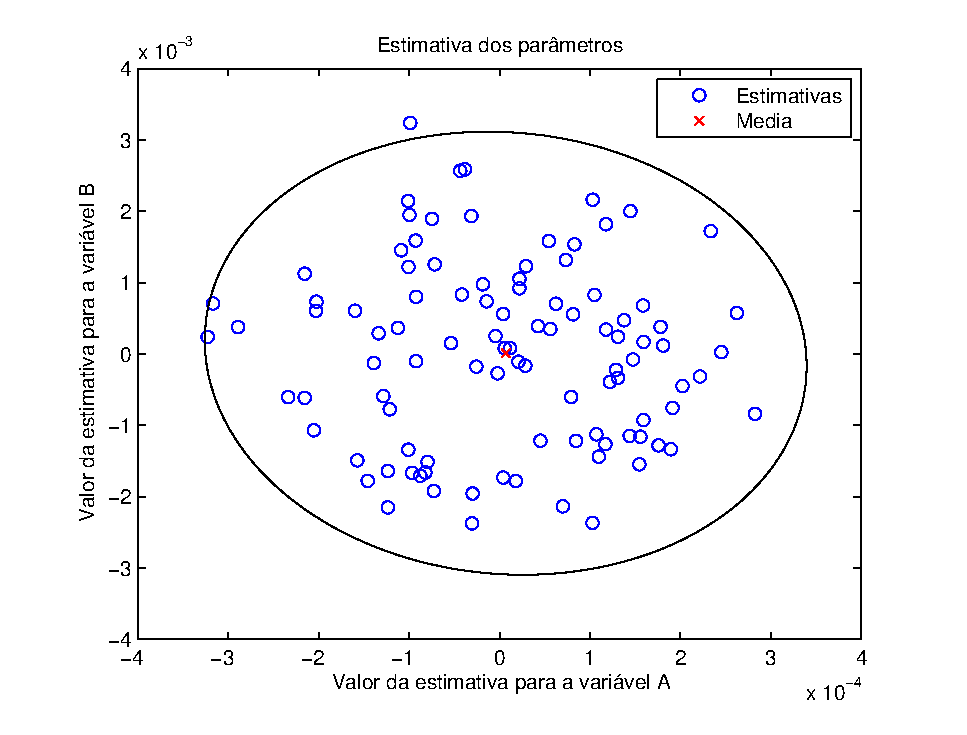
\includegraphics[width=0.8\columnwidth]{figures/si_covar_elipse.eps}
	\caption{Estimativas de um sistema e a regi�o de confian�a para $\chi$ de 95\%}
	\label{fig:si_covar_elipse}
\end{figure}


%===============================================================================
\section{Projeto de Experimento}
\label{sec:si_project_experiments}
%===============================================================================

Projeto de experimentos pode ser entendido como o procedimento para que se escolha o melhor 
sinal de entrada para a identifica��o dos par�metros desejados para o experimento. 
Desta forma muitas vari�veis podem ser levadas em considera��o, refletindo em propriedades que
podem ou n�o ser o foco do projeto de experimentos.

Uma forma de organizar o projeto de experimento � desenvolve-lo como um problema de otimiza��o 
convexa, onde entre muitas vantagens est� o fato de que � poss�vel a utiliza��o de m�todos matem�ticos
para o seu c�lculo e sua formula��o pode ser feita por LMI ({\it{Linear Matrix Inequality}}. Em \cite{jasson}
este t�pico � explorado em mais profundidade, sendo aqui apenas apresentado a sua ideia b�sica.
Este t�pico � abordado na se��o (\ref{sec:si_projec_optimization}).

O projeto de experimento � uma alternativa ao uso de sinais como PRBS ({\it{Pseudo Randon Binary Sequence}}).
A escolha de um sinal mais apropriado para o experimento traz diversas vantagens, que podem ser bastante
significativas para o tempo e esfor�o despendido sobre o projeto do controlador, ou da identifica��o do sistema.
Uma destas vantagens � o tempo de dados coletados, aplicando-se sinais com componentes de frequ�ncia que s�o
mais informativos, tem-se uma efici�ncia maior nos dados amostrados, bastando um montante menor de data, para que
sejam obtidos os mesmos �ndices de qualidade, quando comparado com projetos utilizando sinais mais simples.

%===============================================================================
\subsection{Sinais de entrada mais comumente utilizados}
\label{sec:si_project_signal_input}
%===============================================================================

Como foi apresentado no capitulo (\ref{sec:si_data_persistently_excitation}}) �
poss�vel formar sinais persistentes, apenas adicionando um n�mero suficiente de componentes
de frequ�ncia a fim de que todos os par�metros possam ser estimados. N�o � estranho
que se pense que quanto mais componentes tiver o sinal, melhor. 

Desta maneira, v�rios sinais que podem ser gerados de maneira f�cil e que possuem 
um grande range de componentes de frequ�ncia foram elaborados.

%===============================================================================
\subsubsection{Sinal Bin�rio Rand�mico}
\label{sec:si_project_signal_input_rbs}
%===============================================================================

Um sinal bin�rio por defini��o assume apenas dois valores (0 ou 1). Partindo deste
principio, um sinal bin�rio randomico, � uma sequencia aleat�ria de zeros e uns, que
formam o sinal.


%===============================================================================
\subsubsection{Sinal Bin�rio Pseudo-Rand�mico  - PRBS}
\label{sec:si_project_signal_input_prbs}
%===============================================================================

%===============================================================================
\subsubsection{Ruido Branco Filtrado}
\label{sec:si_project_signal_input_wn_filtered}
%===============================================================================

Um das escolhas mais simples de sinais, � gerar um ruido Gausiano e ent�o filtra-lo com 
algum filtro linear. Desta forma, teoricamente, � poss�vel de se atingir qualquer espectro de
sinal, bastando apenas a correta escolha do filtro. Como este sinal � gerado {\it{off-line}}, 
� poss�vel aplicar filtros n�o causais e eliminar efeitos transientes do sinal, o que
proporciona um comportamento espectral melhor. \cite{campestrini, ljung}

%===============================================================================
\subsection{Modelagem como um problema de otimiza��o}
\label{sec:si_project_optimization}
%===============================================================================

O problema de projeto de experimento pode ser considerado como uma forma geral apresentada em \eqref{eq:si_project_optimization}

\begin{equation}
\begin{matrix}
\underset{\Phi_{\chi_0}}{\text{minimize}} &  & \text{Objetivo}\\ 
\text{Sujeito a:} &  & \text{Requisitos de qualidade}\\ 
 &  & \text{Requisitos de sinais}
\end{matrix}
\label{eq:si_project_optimization}
\end{equation}

De forma geral os requisitos de qualidades s�o fun��es da covari�ncia de $P$. Por esta raz�o � natural usar
o espectro da entrada $\Phi_u$ e eventualmente o espectro cruzado $\Phi_{ue}$ como vari�veis do projeto.
A inclus�o de limita��es nos sinais e sua inclus�o como vari�veis de projeto s�o �teis para evitar que se chegue
em resultados onde a energia de entrada precise ser infinita para se obter os crit�rios desejados, ou largura
de banda que n�o s�o facilmente ating�veis em projetos reais. \cite{jasson}



%===============================================================================
\section{Considera��es Finais}
\label{sec:si_conclusions}
%===============================================================================

Neste capitulo foram apresentados os principais aspectos de um projeto para identifica��o 
de sistemas. Partindo-se da escolha do sinal de excita��o para o experimento onde podemos 
determinar o que � de fundamental import�ncia para a identifica��o e focar os esfor�os para
reduzir ao m�ximo erros nestes aspectos.

Apresentou-se neste quesito de projeto de experimento, a ideia de tornar a escolha do sinal, um
problema de otimiza��o, onde as restri��es s�o as margens de qualidade que desejamos para as
propriedades assint�ticas da estimativa, limita��es de sinais que conseguimos produzir e margens de 
robustez.

Apresentou-se conceitos sobre a escolha do modelo que ser� utilizado para caracterizar o sistema
observado e as propriedades assint�ticas da estimativa para casos onde o sistema real $\mathcal{S}$ n�o
faz parte da fam�lia de modelos $\mathcal{M}$. Esta situa��o onde o sistema real n�o consegue ser
representado completamente pelo modelo adotado, faz com que erros de polariza��o e de vari�ncia 
recaiam sobre a estimativa atingida. Tamb�m foram apresentados os modelos mais comumente utilizados
para a identifica��o de sistemas lineares.

De posse dos dados coletados e da fam�lia de modelos que acredita-se conter o sistema real, � poss�vel, 
com a ajuda de preditores, determinar os par�metros do modelo que descrevem o comportamento do sistema
observado.

Elege-se ent�o uma fun��o dependente do erro entre os dados coletados e os dados gerados pelo preditor. 
Afim de que se tenha a melhor estimativa poss�vel, m�todos de minimiza��o s�o utilizados para que esta 
fun��o dependente do erro, seja minimizada. Obtendo-se assim a melhor estimativa poss�vel 
para aquele conjunto de dados, modelo e crit�rio de minimiza��o escolhidos.

� percept�vel que a identifica��o de um sistema � uma tarefa que depende de um grande conjunto
relativamente grande de de fatores. De um lado isso � extremamente interessante, pois temos liberdade
de escolha e a possibilidade de focar nosso projeto pontos que s�o mais interessantes, em detrimento
de outros que n�o s�o relevantes para o sistema em quest�o. Por outro lado temos um conjunto de
vari�veis que, se n�o compreendidas corretamente, podem tornar este processo algo oneroso e muitas
vezes at� ineficiente.



%===============================================================================



%===============================================================================
\chapter{Virtual Reference Feedback Tunning}
\label{chapter:vfrt}
%===============================================================================
\TODO:: REVER ESTE PARAGRAFO:

Em aplica��es pr�ticas, a descri��o matematica da planta n�o � dispon�vel e o sistema deve ser identificado
baseado nas medidas obtidas deste sistema. Este assunto tem atraido a aten��o de diversos engenheiros de
controle desde 1940 com o pioneiro trabalho de Ziegler e Nichols (1942) com ajuste de controladores PID
industriais. Depois do trabalho de Ziegler e Nichols divesos trabalhos surgiram, muitos em formas de
aperfei�oamento e extens�es das tecnicas ja apresentadas, e algumas com desenvolvimentos em novas dire��es
(\cite{mcmillan1983tuning}, \cite{Haalman1965}). A caracteristica principal destes metodos � que eles podem
ser facilmente utilizados: simples experimentos sobre a planta s�o executados e simples regras 
s�o aplicadas sobre os dados obtidos. O metodo VRFT que ser� abordado aqui tem algumas destas 
caracteristicas, pois s� requer que apenas um experimento seja executado sobre a planta. 
\cite{campi_leccini_savaresi2002}

%===============================================================================
%===============================================================================
\section{Controle baseado em dados}
\label{sec:vrft_control_data_based}
%===============================================================================

O projeto de controladores baseados em dados consiste obter ou ajustar os par�metros de um modelo
para os controladores, baseado nos dados obtidos da planta em an�lise. Os dados utilizados para esta
tarefa s�o basicamente o sinal de entrada e sa�da do sistema.

Como j� foi discutido na se��o (\ref{sec:si_project_experiments}) estes dados podem ser obtidos de
diversas formas. Algumas vezes estas informa��es podem ser a opera��o normal da planta em malha
fechada com a presen�a de algum controlador, situa��o esta que tem um apelo grande em plantas
industriais, onde a parada do processo para levantamento de informa��es � indesej�vel, e muitas
vezes at� invi�vel. Se existe a possibilidade de parar a planta e aplicar-se sinais predeterminados,
o projeto de experimentos pode trazer muitas vantagens.

Seja a esperan�a de um valor $E\left [ \cdot \right ]$ definido por: \cite{ljung}

\begin{equation}
\bar{E}\left [ f(t) \right ]\equiv \lim_{N \to \infty } \frac{1}{N}\sum_{t=1}^{N}E\left [ f(t)
\right]
\label{eq:vrft_db_hope}
\end{equation}

Um sinal � dito quasi-estacionario se a m�dia e autocorrela��o do mesmo convergem para um valor
finito quando o tamanho da amostra cresce, conforme defini��o a seguir: \cite{campestrini}


\begin{defn}
\cite{ljung}

Um Sinal $s(t)$ � um processo quasi-estacionario se:
\begin{itemize}
	\item $\bar{E}\left [ s(t) \right ] = \mid m_s \mid \le C, \;\forall t$;
	\item $\bar{E}\left [ s(t)s(r) \right ] = \mid R_s(t,s) \mid \le C, \;\forall t,r$;
	\item $\lim_{N \to \infty}\frac{1}{N}\sum_{t=1}^{N}R_s(t, t-\tau)=R_s(\tau), \; \forall \tau$,
\end{itemize}
Onde $m_s(t)$ � o valor m�dio do sinal $s(t)$ e $R_s(t,r)$ � a covari�ncia do sinal $s$ nos
instantes $t$ e $r$.
\end{defn}

O ruido � um processo quasi-estacionario, que pode ser descrito como $\nu(t)=H_0(z)e(t)$, onde
$e(t)$ � ruido branco com vari�ncia $\sigma_e^2$. Ambas fun��es de transfer�ncia, $G(z)$ e $H(z)$,
s�o racionais e causais. Assume-se que $H(\infty)=1$, ou seja, a resposta impulsiva do filtro
$H_0(z)$ satisfaz $h(0)=1$. \cite{campestrini}

Na Figura (\ref{fig:vrft_db_control_loop}) � apresentado uma malha de controle onde o controlador
$C(z, \rho) \in \mathcal{C}$ onde $ \mathcal{C}$ � a classe de controladores definida pelo usu�rio.

\begin{figure}[htbp]
\center
\scalebox{1} % Change this value to rescale the drawing.
{
\begin{pspicture}(0,-1.1092187)(9.868125,1.1292187)
\pscircle[linewidth=0.04,dimen=outer](1.4,-0.08921875){0.2}
\psframe[linewidth=0.04,dimen=outer](4.4,0.31078124)(2.6,-0.48921874)
\psframe[linewidth=0.04,dimen=outer](7.2,0.31078124)(5.6,-0.48921874)
\pscircle[linewidth=0.04,dimen=outer](8.4,-0.08921875){0.2}
\psline[linewidth=0.04cm,arrowsize=0.05291667cm 2.0,arrowlength=1.4,arrowinset=0.4]{->}(0.0,-0.08921875)(1.2,-0.08921875)
\psline[linewidth=0.04cm,arrowsize=0.05291667cm 2.0,arrowlength=1.4,arrowinset=0.4]{->}(1.6,-0.08921875)(2.6,-0.08921875)
\psline[linewidth=0.04cm,arrowsize=0.05291667cm 2.0,arrowlength=1.4,arrowinset=0.4]{->}(4.4,-0.08921875)(5.6,-0.08921875)
\psline[linewidth=0.04cm,arrowsize=0.05291667cm 2.0,arrowlength=1.4,arrowinset=0.4]{->}(7.2,-0.08921875)(8.2,-0.08921875)
\psline[linewidth=0.04cm,arrowsize=0.05291667cm 2.0,arrowlength=1.4,arrowinset=0.4]{->}(8.4,0.7107813)(8.4,0.11078125)
\psline[linewidth=0.04cm,arrowsize=0.05291667cm 2.0,arrowlength=1.4,arrowinset=0.4]{->}(8.6,-0.08921875)(9.8,-0.08921875)
\psline[linewidth=0.04cm,arrowsize=0.05291667cm 2.0,arrowlength=1.4,arrowinset=0.4]{<-}(1.4,-0.28921875)(1.4,-1.0892187)
\psline[linewidth=0.04cm](1.4,-1.0892187)(9.2,-1.0892187)
\psline[linewidth=0.04cm](9.2,-1.0892187)(9.2,-0.08921875)
\usefont{T1}{ptm}{m}{n}
\rput(1.1126562,0.22078125){+}
\usefont{T1}{ptm}{m}{n}
\rput(8.112657,0.22078125){+}
\usefont{T1}{ptm}{m}{n}
\rput(8.112657,-0.37921876){+}
\usefont{T1}{ptm}{m}{n}
\rput(1.6473438,-0.37921876){-}
\usefont{T1}{ptm}{m}{n}
\rput(0.47,0.21078125){\small $r(t)$}
\usefont{T1}{ptm}{m}{n}
\rput(3.59,-0.08921875){\small $C(z, \rho)$}
\usefont{T1}{ptm}{m}{n}
\rput(6.36,-0.10921875){\small $G_0(z)$}
\usefont{T1}{ptm}{m}{n}
\rput(5.11,0.21078125){\small $u(t)$}
\usefont{T1}{ptm}{m}{n}
\rput(2.21,0.21078125){\small $\xi(t)$}
\usefont{T1}{ptm}{m}{n}
\rput(8.48,0.93078125){\small $\nu(t)$}
\usefont{T1}{ptm}{m}{n}
\rput(9.3,0.21078125){\small $y(t)$}
\end{pspicture} 
}
\caption{Rede neural recorrentes.}
\label{fig:vrft_db_control_loop}
\end{figure}

A equa��o \eqref{eq:vrft_db_closed_loop} descreve o comportamento do sistema da Figura
(\ref{fig:vrft_db_control_loop}).

\begin{equation}
T(z, \rho)=\frac{C(z,\rho)G_0(z)}{1+C(z,\rho)G_0(z)}
\label{eq:vrft_db_closed_loop}
\end{equation}

Controle baseado em dados pode ser dividido em dois grupos principais: m�todos iterativos onde
experimentos s�o realizados sobre o sistema atualizando-se o controlador, o processo ent�o � repetido
at� que se atinja um valor minimo para a fun��o custo deste sistema. O segundo grupo � o de m�todos
n�o iterativos, onde apenas com um experimento, ou um conjunto de dados, os par�metros do
controlador s�o estimados.



%===============================================================================
\section{Iterative feedback tuning}
\label{sec:vrft_control_ift}
%===============================================================================

O m�todo IFT utiliza um algoritmo iterativo para minimizar uma fun��o custo $H_2$. O m�todo
considera que o sistema � controlado por um controlador com dois graus de liberdade:

\begin{equation}
u(t)=C_r(z)r(t)-C_y(z)y(t)
\label{eq:vrft_db_ift_controller}
\end{equation}

Na Figura (\ref{fig:vrft_db_ift}) � apresentado a organiza��o dos blocos dos controladores
apresentados em \eqref{eq:vrft_db_ift_controller}, $C_r(z)$ e $C_y(z)$. O controlador pode ser
entendido como o conjunto destes dois:\cite{ift_theory_and_applications}

\begin{equation}
C(z) \equiv  \left \{ C_r(z),\, C_y(z)  \right \} 
\nonumber
\end{equation}

\begin{figure}[htbp]
\center
\scalebox{1} % Change this value to rescale the drawing.
{
\begin{pspicture}(0,-1.68)(9.48,1.72)
\usefont{T1}{ptm}{m}{n}
\rput(7.691875,1.5215625){\small $\nu(t)$}
\pscircle[linewidth=0.04,dimen=outer](4.0,0.32){0.2}
\pscircle[linewidth=0.04,dimen=outer](8.0,0.32){0.2}
\psframe[linewidth=0.04,dimen=outer](6.8,0.72)(5.2,-0.08)
\psframe[linewidth=0.04,dimen=outer](2.8,0.72)(1.2,-0.08)
\psframe[linewidth=0.04,dimen=outer](6.8,-0.88)(5.2,-1.68)
\psline[linewidth=0.04cm,arrowsize=0.05291667cm 2.0,arrowlength=1.4,arrowinset=0.4]{->}(0.0,0.32)(1.2,0.32)
\psline[linewidth=0.04cm,arrowsize=0.05291667cm 2.0,arrowlength=1.4,arrowinset=0.4]{->}(2.8,0.32)(3.8,0.32)
\psline[linewidth=0.04cm,arrowsize=0.05291667cm 2.0,arrowlength=1.4,arrowinset=0.4]{->}(4.2,0.32)(5.2,0.32)
\psline[linewidth=0.04cm,arrowsize=0.05291667cm 2.0,arrowlength=1.4,arrowinset=0.4]{->}(6.8,0.32)(7.8,0.32)
\psline[linewidth=0.04cm,arrowsize=0.05291667cm 2.0,arrowlength=1.4,arrowinset=0.4]{->}(8.2,0.32)(9.2,0.32)
\psline[linewidth=0.04cm,arrowsize=0.05291667cm 2.0,arrowlength=1.4,arrowinset=0.4]{<-}(6.8,-1.28)(8.0,-1.28)
\psline[linewidth=0.04cm](8.0,-1.28)(8.0,0.12)
\psline[linewidth=0.04cm,arrowsize=0.05291667cm 2.0,arrowlength=1.4,arrowinset=0.4]{<-}(4.0,0.12)(4.0,-1.28)
\psline[linewidth=0.04cm](4.0,-1.28)(5.2,-1.28)
\usefont{T1}{ptm}{m}{n}
\rput(8.911875,0.5215625){\small $y(t)$}
\usefont{T1}{ptm}{m}{n}
\rput(0.481875,0.5215625){\small $r(t)$}
\usefont{T1}{ptm}{m}{n}
\rput(1.901875,0.3215625){\small $C_r(z)$}
\usefont{T1}{ptm}{m}{n}
\rput(5.951875,0.3215625){\small $G_0(z)$}
\usefont{T1}{ptm}{m}{n}
\rput(5.931875,-1.2784375){\small $C_y(z)$}
\usefont{T1}{ptm}{m}{n}
\rput(4.721875,0.7215625){\small $u(t)$}
\psline[linewidth=0.04cm,arrowsize=0.05291667cm 2.0,arrowlength=1.4,arrowinset=0.4]{->}(8.0,1.32)(8.0,0.52)
\usefont{T1}{ptm}{m}{n}
\rput(4.2592187,0.1315625){-}
\end{pspicture} 
}
\caption{Diagrama de bloco do sistema utilizado na identifica��o IFT.}
\label{fig:vrft_db_ift}
\end{figure}

\begin{equation}
J(\rho)=\frac{1}{2N}E\left [ \sum_{t=1}^{N}(L_y \tilde{y}_t(\rho))^2 +\lambda  \sum_{t=1}^{N}(L_u
u_t(\rho))^2 \right ]
\label{eq:vrft_db_ift_j_cost}
\end{equation}








\begin{figure}[htbp]
\center
\scalebox{1} % Change this value to rescale the drawing.
{
\begin{pspicture}(0,-1.4292188)(9.02,1.4692187)
\pscircle[linewidth=0.04,linestyle=dashed,dash=0.16cm 0.16cm,dimen=outer](1.4,0.97078127){0.2}
\psframe[linewidth=0.04,linestyle=dashed,dash=0.16cm 0.16cm,dimen=outer](4.8,1.3707813)(3.0,0.57078123)
\psframe[linewidth=0.04,dimen=outer](7.6,1.3707813)(6.0,0.57078123)
\psline[linewidth=0.04cm,arrowsize=0.05291667cm 2.0,arrowlength=1.4,arrowinset=0.4]{->}(0.0,0.97078127)(1.2,0.97078127)
\psline[linewidth=0.04cm,linestyle=dashed,dash=0.16cm 0.16cm,arrowsize=0.05291667cm 2.0,arrowlength=1.4,arrowinset=0.4]{->}(1.6,0.97078127)(3.0,0.97078127)
\psline[linewidth=0.04cm,arrowsize=0.05291667cm 2.0,arrowlength=1.4,arrowinset=0.4]{->}(4.8,0.97078127)(6.0,0.97078127)
\psline[linewidth=0.04cm](7.6,0.97078127)(9.0,0.97078127)
\psline[linewidth=0.04cm,linestyle=dashed,dash=0.16cm 0.16cm,arrowsize=0.05291667cm 2.0,arrowlength=1.4,arrowinset=0.4]{<-}(1.4,0.7707813)(1.4,-0.02921875)
\psline[linewidth=0.04cm,linestyle=dashed,dash=0.16cm 0.16cm](1.4,-0.02921875)(8.4,-0.02921875)
\psline[linewidth=0.04cm,linestyle=dashed,dash=0.16cm 0.16cm](8.4,-0.02921875)(8.4,0.97078127)
\usefont{T1}{ptm}{m}{n}
\rput(1.1126562,1.2807813){+}
\usefont{T1}{ptm}{m}{n}
\rput(1.6473438,0.68078125){-}
\usefont{T1}{ptm}{m}{n}
\rput(0.47,1.2707813){\small $r(t)$}
\usefont{T1}{ptm}{m}{n}
\rput(3.99,0.97078127){\small $C(z, \rho)$}
\usefont{T1}{ptm}{m}{n}
\rput(6.76,0.9507812){\small $G_0(z)$}
\usefont{T1}{ptm}{m}{n}
\rput(5.51,1.2707813){\small $u(t)$}
\usefont{T1}{ptm}{m}{n}
\rput(2.25,1.2707813){\small $\bar{e}(t)$}
\usefont{T1}{ptm}{m}{n}
\rput(8.3,1.2707813){\small $y(t)$}
\psframe[linewidth=0.04,dimen=outer](6.0,-0.62921876)(3.8,-1.4292188)
\usefont{T1}{ptm}{m}{n}
\rput(4.91,-1.0492188){\small $M^{-1}(z)$}
\psline[linewidth=0.04cm](9.0,0.97078127)(9.0,-1.0292188)
\psline[linewidth=0.04cm](9.0,-1.0292188)(6.0,-1.0292188)
\psline[linewidth=0.04cm](3.8,-1.0292188)(0.0,-1.0292188)
\psline[linewidth=0.04cm](0.0,-1.0292188)(0.0,0.97078127)
\end{pspicture} 
}
\caption{Rede neural recorrentes.}
\label{fig:nl_models_neural_recurrent}
\end{figure}

% ===============================================================================
\section{VRFT}
\label{sec:vrft_vrft}
% ===============================================================================

VRFT do ingl�s {\it{Virtual reference feedback tuning}} � um m�todo direto para identifica��o de
controladores, ou seja, n�o � necess�rio o conhecimento ou identifica��o da planta para que este m�todo seja
utilizado. Desta forma pode ser utilizado com apenas um conjunto de dados, n�o necessitando de experimentos
espec�ficos. O procedimento procura pelo ponto �timo do crit�rio escolhido para a identifica��o do
controlador. \cite{campi_savaresi2000}

Diferentemente de m�todos iterativos, o VRFT n�o recai sobre minimos locais, sempre procurando o m�nimo global
do crit�rio escolhido. � importante salientar que o valor de minimo global encontrado � relativo. O valor
encontrado pelo m�todo � um minimo dentro das limita��es de qualidade e exitabilidade do sinal utilizado para
se adquirir os dados utilizados no processo.

Assume-se que a planta do sistema � {\it{linear}} SISO ({\it{single input single output}}) de tempo discreto
descrito pela fun��o de transfer�ncia racional $G(z)$. Tal que esta fun��o de transfer�ncia � desconhecida e
tem-se apenas acesso ao conjunto de dados coletados do experimento.
\cite{campi_leccini_savaresi2002}

O controlador a ser identificado pode ser parametrizado como em \eqref{eq:vrft_method_controller}

\begin{equation}
C(z,\theta)=\beta^T(z)\theta
\label{eq:vrft_method_controller}
\end{equation}

Onde $\beta(z) = \left [ \beta_1(z)\;\; \beta_2(z)\;\; \cdots \;\; \beta_n(z)\right ]^T$ � um vetor
linear de fun��es de transfer�ncias de tempo discreto e $\theta = \left [ \vartheta_1 \;\;
\vartheta_2 \;\; \cdots \;\; \vartheta_n \right ]^T \in \mathcal{R}^n$ � um vetor $n$-dimensional de
par�metros a serem estimados.

O problema de identifica��o do controlador consiste em encontrar um $\hat{\theta}$ que minimize o
crit�rio performance \eqref{eq:vrft_method_cost_func} que � dependente do modelo de refer�ncia
escolhido.

\begin{equation}
J_{MR}(\theta) = \left \| \left ( \frac{G(z)C(z,\theta)}{1+G(z)C(z,\theta)} -M(z) \right )W(z)
\right \|_2^2 
\label{eq:vrft_method_cost_func}
\end{equation} 

Sendo $M(z)$ o modelo de refer�ncia a ser atingido em malha fechada quando o controlador
obtido � aplicado sobre a planta e $W(z)$ � uma matriz para pondera��o escolhida pelo usu�rio.

Como j� mencionado, VRFT � um m�todo {\it{direto}}, onde os dados coletados da planta s�o utilizados
diretamente para identificar o controlador e n�o h� necessidaade de identifica��o da planta para
ent�o haver a identifica��o do controlador. M�todos diretos s�o conceitualmente mais naturais que
os indiretos, mas mesmo com o apelo que estes m�todos possuem, apenas alguns m�todos genuinamente
diretos s�o encontrados na literatura, dois destes s�o VRFT e IFT (se��o
(\ref{sec:vrft_control_ift})), mesmo estes dois m�todos pertencendo uma a mesma classe de m�todos,
algumas diferen�as s�o ressaltadas: \cite{campi_savaresi2000}

\begin{itemize}
	\item {\it{IFT}} � baseado em um m�todos de gradiente decrescente e al�m disso � uma t�cnica
	iterativa. Usualmente este m�todo converge para o minimo local mais pr�ximo das condi��es iniciais.
	Ele requer experimentos espec�ficos sobre a planta, com entradas especificas.
	\item {\it{VRFT}} � um procedimento n�o iterativo que procura pelo minimo global do crit�rio de
	performance \eqref{eq:vrft_method_cost_func}. Este m�todo n�o requer experimentos espec�ficos sobre
	a planta, podendo inclusive utilizar os dados do funcionamento normal da planta.
\end{itemize}

%===============================================================================
\subsection{O m�todo}
\label{sec:vrft_framework}
%===============================================================================

Nesta se��o ser� apresentado uma breve descri��o de como o algoritmo para obten��o do controlador
utilizando o m�todo VRFT � formulado. Para maiores detalhes e discuss�es aprofundadas �
indicada a leitura de \cite{campi_savaresi2000}, 
\cite{campi_leccini_savaresi2002} e \cite{campestrini_nonminumum_phase}.

Suponha que o controlador $C(z, \theta)$ resulta um sistema em malha fechada cuja fun��o de
transfer�ncia � dada por $M(z)$. Desta forma, se $M(z)$ for alimentado com qualquer sinal $r(t)$,
sua sa�da ser� $M(z)r(t)$. Uma premissa para que o sistema em malha fechada tenha a mesma
fun��o de transfer�ncia que o modelo de refer�ncia � que a sa�da dos dois seja a mesma para um dado
sinal $\bar{r}(t)$.

Baseado no sinal medido $y(t)$, considera-se um sinal $\bar{r}(t)$ tal que $M(z)\bar{r}(t)=y(t)$.
Esta refer�ncia � conhecida como {\it{virtual}} pois ela n�o existe e n�o foi utilizada para gerar o
sinal $y(t)$. A figura (\ref{fig:vrft_method_cl}) apresenta o sistema em malha fechada e os sinais
utilizados.

\begin{figure}[htbp]
\center
%\scalebox{1} % Change this value to rescale the drawing.
%{
\begin{pspicture}(0,-1.4292188)(9.02,1.4692187)
\pscircle[linewidth=0.04,linestyle=dashed,dash=0.16cm 0.16cm,dimen=outer](1.4,0.97078127){0.2}
\psframe[linewidth=0.04,linestyle=dashed,dash=0.16cm 0.16cm,dimen=outer](4.8,1.3707813)(3.0,0.57078123)
\psframe[linewidth=0.04,dimen=outer](7.6,1.3707813)(6.0,0.57078123)
\psline[linewidth=0.04cm,arrowsize=0.05291667cm 2.0,arrowlength=1.4,arrowinset=0.4]{->}(0.0,0.97078127)(1.2,0.97078127)
\psline[linewidth=0.04cm,linestyle=dashed,dash=0.16cm 0.16cm,arrowsize=0.05291667cm 2.0,arrowlength=1.4,arrowinset=0.4]{->}(1.6,0.97078127)(3.0,0.97078127)
\psline[linewidth=0.04cm,arrowsize=0.05291667cm 2.0,arrowlength=1.4,arrowinset=0.4]{->}(4.8,0.97078127)(6.0,0.97078127)
\psline[linewidth=0.04cm](7.6,0.97078127)(9.0,0.97078127)
\psline[linewidth=0.04cm,linestyle=dashed,dash=0.16cm 0.16cm,arrowsize=0.05291667cm 2.0,arrowlength=1.4,arrowinset=0.4]{<-}(1.4,0.7707813)(1.4,-0.02921875)
\psline[linewidth=0.04cm,linestyle=dashed,dash=0.16cm 0.16cm](1.4,-0.02921875)(8.4,-0.02921875)
\psline[linewidth=0.04cm,linestyle=dashed,dash=0.16cm 0.16cm](8.4,-0.02921875)(8.4,0.97078127)
\usefont{T1}{ptm}{m}{n}
\rput(1.1126562,1.2807813){+}
\usefont{T1}{ptm}{m}{n}
\rput(1.6473438,0.68078125){-}
\usefont{T1}{ptm}{m}{n}
\rput(0.47,1.2707813){\small $\bar{r}(t)$}
\usefont{T1}{ptm}{m}{n}
\rput(3.99,0.97078127){\small $C(z, \rho)$}
\usefont{T1}{ptm}{m}{n}
\rput(6.76,0.9507812){\small $G_0(z)$}
\usefont{T1}{ptm}{m}{n}
\rput(5.51,1.2707813){\small $u(t)$}
\usefont{T1}{ptm}{m}{n}
\rput(2.25,1.2707813){\small $e(t)$}
\usefont{T1}{ptm}{m}{n}
\rput(8.3,1.2707813){\small $y(t)$}
\psframe[linewidth=0.04,dimen=outer](6.0,-0.62921876)(3.8,-1.4292188)
\usefont{T1}{ptm}{m}{n}
\rput(4.91,-1.0492188){\small $M^{-1}(z)$}
\psline[linewidth=0.04cm](9.0,0.97078127)(9.0,-1.0292188)
\psline[linewidth=0.04cm](9.0,-1.0292188)(6.0,-1.0292188)
\psline[linewidth=0.04cm](3.8,-1.0292188)(0.0,-1.0292188)
\psline[linewidth=0.04cm](0.0,-1.0292188)(0.0,0.97078127)
\end{pspicture} 
%}
\caption{dlkjhsfjdhf kljh dfh sdlf}
\label{fig:vrft_method_cl}
\end{figure}

O sinal $e(t)$ � o erro entre os sinais $y(t)$ e $\bar{r}(t)$. Sabe-se que quando a planta �
alimentada com o sinal $u(t)$, o sinal $y(t)$ � obtido. Em um controlador, quando este �
alimentado com o sinal $e(t)$, o sinal $u(t)$ � obtido. A tarefa do m�todo VRFT � encontrar este
controlador, como os sinais $u(t)$ e $e(t)$ s�o conhecidos, a tarefa reduz-se a um problema de
identifica��o. Comumente, usa-se um pr�-filtro nos dados coletados. A ideia principal do uso deste
filtro ser� explicada posteriormente na se��o (\ref{sec:vrft_framework_filter}). 

O algoritmo pode ser descrito pelos passos a seguir \cite{campi_savaresi2000}:

\begin{enumerate}
	\item Filtram-se os sinais de entrada e sa�da com algum filtro $L(z)$:

\begin{equation}
y_L (t)=L(z)y(t), \;\;\; u_L (t)=L(z)u(t) 
\label{eq:vrft_method_algorithm_filter_io}
\end{equation}

\item Encontra-se um sinal de refer�ncia $\bar{r}_L (t)$ no qual a sa�da do modelo de refer�ncia
$M(z)$ seja exatamente $y_L (t)$ quando alimentado pelo sinal:

\begin{equation}
y_L (t)=M(z) \bar{r}_L (t)
\label{eq:vrft_method_algorithm_ref}
\end{equation}

\item Selecione o vetor de parametros do controlador $\hat{\theta}$ que minimize o crit�rio
\eqref{eq:vrft_method_algorithm_criter}

\begin{equation}
J_{VR}^N(\theta)=\frac{1}{N}\sum_{t=1}^{N}(u_L(t)-\varphi_L^T(t)\theta)^2
\label{eq:vrft_method_algorithm_criter}
\end{equation}

\begin{equation}
\varphi_L(t)=\beta(z)e_L(t)
\nonumber
\end{equation}

Desde que \eqref{eq:vrft_method_algorithm_criter} seja quadr�tica em $\theta$ o vetor de parametros
$\hat{\theta}$ que minimizam esta fun��o custo podem ser calculados com
\eqref{eq:vrft_method_algorithm_result}.


\begin{equation}
\hat{\theta}= \left [ \sum_{t=1}^{N}\varphi_L(t) \varphi_L(t)^T\right ]^{-1}
\sum_{t=1}^{N}\varphi_L(t) u_L(t)
\label{eq:vrft_method_algorithm_result}
\end{equation}

\end{enumerate}

%===============================================================================
\subsubsection{Filtro $L(z)$}
\label{sec:vrft_framework_filter}
%===============================================================================

Considerando a fun��o custo $J_{MR}(\theta)$ apresentada em \eqref{eq:vrft_method_cost_func} e o
crit�rio do m�todo de refer�ncia virtual $J_{VR}(\theta)$ apresentado em
\eqref{eq:vrft_method_algorithm_criter} serem diferentes. A escolha correta do filtro $L(z)$
propicia que estas duas equa��es tenham m�nimos muito proximos.
\cite{campi_leccini_savaresi2002}

A utiliza��o do filtro � de grande import�ncia em situa��es onde a escolha do modelo $\mathcal{C}(z,
\theta)$ n�o consegue representar a totalidade do controlador �timo ($C_0(z)$) que quando aplicado em conjunto com a
planta proporciona a exata resposta desejada pela escolha de $M(z)$.

\begin{equation}
C_0(z) \notin \mathcal{C}(z, \theta)
\nonumber
\end{equation}

O crit�rio $J_{MR}(\theta)$ pode ser reescrito utilizando-se o controlador �timo $C_0(z)$ como em 
\eqref{eq:vrft_method_filter_cost_func}

\begin{equation}
J_{MR}(\theta)= \frac{1}{2\pi} \int_{-\pi}^{\pi} \frac{\left | G \right |^2 \left | W \right |^2 }
{\left | 1+GC(\theta) \right |^2} 
\frac{\left |C(\theta)-C_0  \right |^2}{\left |1+GC_0 \right |^2}d\omega 
\label{eq:vrft_method_filter_cost_func}
\end{equation}

Considerando que $J_{VR}^N$ seja conhecido, quando a quantidade de dados cresce: $N \to \infty$
tem-se \eqref{eq:vrft_method_filter_criter_assim}. 

\begin{equation}
J_{VR}^N(\theta) \to J_{VR}(\theta = E \left [ (u_L(t) - C(z, \theta)e_L(t))^2\right ])
\label{eq:vrft_method_filter_criter_assim}
\end{equation}

Utilizando as defini��es de $u_L(t)$, $e_L(t)$ e dada a defini��o de $C_0(z)$ juntament com o
teorema de Perseval \cite{ljung}, o crit�rio assint�tico \eqref{eq:vrft_method_filter_criter_assim}
tem sua representa��o como em \eqref{eq:vrft_method_filter_criter_vr}

\begin{equation}
J_{VR}(\theta)= \frac{1}{2\pi} \int_{-\pi}^{\pi} \left | G \right |^2 \left | C(\theta)-C_0 \right
|^2 \left | 1-M \right |^2 \frac{\left | L \right |^2}{\left | M \right |^2} \Phi_u \; d\omega
\label{eq:vrft_method_filter_criter_vr}
\end{equation}

Onde $\Phi_u $ � a densidade do espectro do sinal $u(t)$.

Para o caso onde $C_0 \in C(z, \theta)$ a escolha de $L(z)$ n�o afeta o resultado, usualmente
escolhe-se ent�o $L(z)=1$. Caso o controlador n�o consiga ser representado pelo modelo, a escolha de
$L(z)$ pode ser feita por:

\begin{equation}
\left | L \right | ^2 = \left | 1-M \right | ^2 \left | M \right | ^2 \left | W \right | ^2 \frac{1}
{\Phi_u}, \;\;\; \forall \omega \in [-\pi; \pi].
\label{eq:vrft_method_filter_l}
\end{equation}

Obtem-se com a utiliza��o do filtro, uma estimativa onde o erro de polariza��o � minimizado.
%===============================================================================
\subsubsection{VRFT e dados corrompidos por ruido}
\label{sec:vrft_framework_noise}
%===============================================================================

Todos os equacionamentos at� aqui apresentadso, consideraram que o sistema n�o seja afetado por
ruido. Nesta se��o ser� apresentado brevemente o comportamento do m�todo quando o sinal $y(t)$ �
corrompido por um ruido aditivo como:

\begin{equation}
\tilde{y}(t)=G(z)u(t) + \xi(t)
\label{eq:vrft_framework_noise_y}
\end{equation}

Assume-se que o sinal $u(t)$ e $\xi(t)$ sejam descorrelacionados e tamb�m que os dados s�o coletados
com a planta trabalhando em la�o aberto. \cite{campi_leccini_savaresi2002}. Para a id�ia extendida
de dados coletados com a planta em la�o fechado, uma explica��o mais detalhada pode ser encontrada
em \cite{lecchini}.

Ao aplicar o algoritmo descrito na se��o (\ref{sec:vrft_framework}) com dados sugeitos a ruidos, o
resultado obtido possui erro de polariza��o (se��o (\ref{sec:si_par_estim_uncertanties})). Isso pode
ser compreendido analizando a express�o do crit�rio $J_{VR}(\theta)$ quando utiliza-se o sinal
$\tilde{y}(t)$:


\begin{equation}
J_{VR}(\theta)= \frac{1}{2\pi} \int_{-\pi}^{\pi} \left [ \left | G \right |^2 \left | C(\theta)-C_0
\right |^2 \left | 1-M \right |^2 \frac{\left | L \right |^2}{\left | M \right |^2} \Phi_u +\frac{\left | 
C(\theta) \right |^2}{\left | G \right |^2 \left | C_0 \right |^2}\left | L \right |^2\Phi _d
\right ] \; d\omega
\label{eq:vrft_framework_noise_vr}
\end{equation}

Onde $\Phi_d$ � a densidade do espectro do ruido.

Para que haja rejei��o a este rudo no m�todo, em \cite{campi_leccini_savaresi2002} foi sugerido a
adi��o da vari�vel instrumental $\zeta(t)$. Em \eqref{eq:vrft_framework_noise_iv} apresenta-se o
regressor deste instrumento:

\begin{equation}
\tilde{\varphi }_L=\beta(z)L(z)\left ( M(z)^{-1}-1 \right )\tilde{y}(t)
\label{eq:vrft_framework_noise_iv}
\end{equation}

Os parametros do controlador $\hat{\theta}^{IV}_N $ podem ent�o ser calculados como em
\eqref{eq:vrft_framework_noise_theta_iv}.

\begin{equation}
\hat{\theta}_{N}^{IV}=\left [ \sum_{t=1}^{N}\zeta(t) \tilde{\varphi}_L(t)^T \right ]^{-1}\left [ 
\sum_{t=1}^{N}\zeta(t)u_L(t) \right ]
\label{eq:vrft_framework_noise_theta_iv}
\end{equation}

S�o propostas duas alternativas para a escolha da vari�vel instrumental. A primeira garante
assimtoticamente que $\hat{\theta}^{IV}= \hat{\theta}$, entretanto um experimento adicional �
requisitado, o segundo n�o garante rigorosamente $\hat{\theta}^{IV}= \hat{\theta}$, mas o erro
esperado � pequeno, al�m disso um segundo experimento n�o � necess�rio.
\cite{campi_leccini_savaresi2002}

\begin{itemize}
	\item {\it{Experimento Repetido:}} Executa-se um segundo experimento com a mesma entrada $u(t)$,
	adquirindo-se a saida $\tilde{y}(t)'$. Como o rudio entre um experimento e outro � independente,
	$\tilde{y}(t)$ e $\tilde{y}(t)'$ ser�o diferentes. Obtem-se ent�o a variavel instrumental:
	
	\begin{equation}
	\zeta(y)=\beta(z)L(z)\left ( M(z)^{-1}-1 \right )\tilde{y}(t)'
	\nonumber
	\end{equation}
	
	\item {\it{Identifica��o da planta:}} Identifica-se um modelo para a planta $\hat{G}(z)$ a partir
	do conjunto de dados $\left \{ u(t), \; \tilde{y}(t) \right \}_{t=1,..., N}$  e ent�o gera-se o
	sinal simulado $\hat{y}=\hat{G}u(t)$, obtendo a variavel instrumental como:

	\begin{equation}
	\zeta(y)=\beta(z)L(z)\left ( M(z)^{-1}-1 \right )\hat{y}(t)
	\nonumber
	\end{equation}
	
	Devido as incertezas na estimativa de $\hat{G}(z)$, este segundo m�todo n�o garante que a
	estimativa tenda assimtoticamente a $\hat{\theta}$.
	
\end{itemize}

%===============================================================================
\subsection{Exemplos ilustrativos}
\label{sec:vrft_examples}
%===============================================================================

Nesta se��o ser�o apresentados alguns exemplos ilustrativos da utiliza��o do m�todo do VFRT. Para isso ser�o
utilizados sistemas lineares modelados utilizando modelos ARX e BJ quando o controlador $C(z, \rho)$ faz parte
da classe de controladores que representa completamente o controlador ideal. Sendo este o controlador que
consegue levar o sistema para o comportamento escolhido $M(z)$.

Nas identifica��es apresentadas a seguir ser� sempre utilizado um sina PRBS (Se��o
(\ref{sec:si_project_signal_input_prbs})) de ordem 7.

%===============================================================================
\subsubsection{Controlador PI - sistema Box-Jenkins}
\label{sec:vrft_examples_pi_bj}
%===============================================================================

Para um sistema onde $G_0(z)$ e $H_0(z)$ podem ser definidos como:

\begin{equation}
G_{ 0 }(z)=\frac { 0.5 }{ z-0.85 } ,\quad \quad \quad H_{ 0 }(z)=\frac { z }{
z-0.4 } 
\nonumber
\end{equation}

Este sistema pode ser compreendido como um sistema {\it{Box-Jenkins}} (BJ)
(Tabela (\ref{table:si_modeling_models})). Deseja-se que o sistema em malha
fechada comporte-se o mais pr�ximo poss�vel do modelo apresentado em
\eqref{eq:vrft_methos_ex_bj_M}.

\begin{equation}
M(z)=\frac { 0.4 }{ z-0.6 }
\label{eq:vrft_methos_ex_bj_M}
\end{equation}

Tem-se assim que o controlador ideal, aquele que ao ser inserido no sistema em
malha fechada apresentado na Figura (\ref{fig:vrft_db_control_loop}) propicia o
comportamento descrito por \eqref{eq:vrft_methos_ex_bj_M} �:

\begin{equation}
C_d(z)=\frac { 0.8(z - 0.85) }{ z-1 }
\label{eq:vrft_methos_ex_bj_cd}
\end{equation}

Observa-se que este controlador pode ser representado como um controlador
{\it{PI}} como em \eqref{eq:vrft_methos_ex_bj_c}. 

\begin{equation}
C(z, \rho)=\frac { \rho_1 z +\rho_2}{ z-1 }
\label{eq:vrft_methos_ex_bj_c}
\end{equation}

Utilizando o m�todo do VRFT para identifica��o do controlador quando este est� submetido a um ruido $\sigma
_\upsilon ^2=0.005$ obtem-se a estimativas dos parametro s $\rho_1$ e $\rho_2$ apresentados na Figura
(\ref{fig:vrft_bj_M10_var005}) com um resultado de 100 simula��es de 2540 amostras cada.

\begin{figure}[htbp]
	\center
	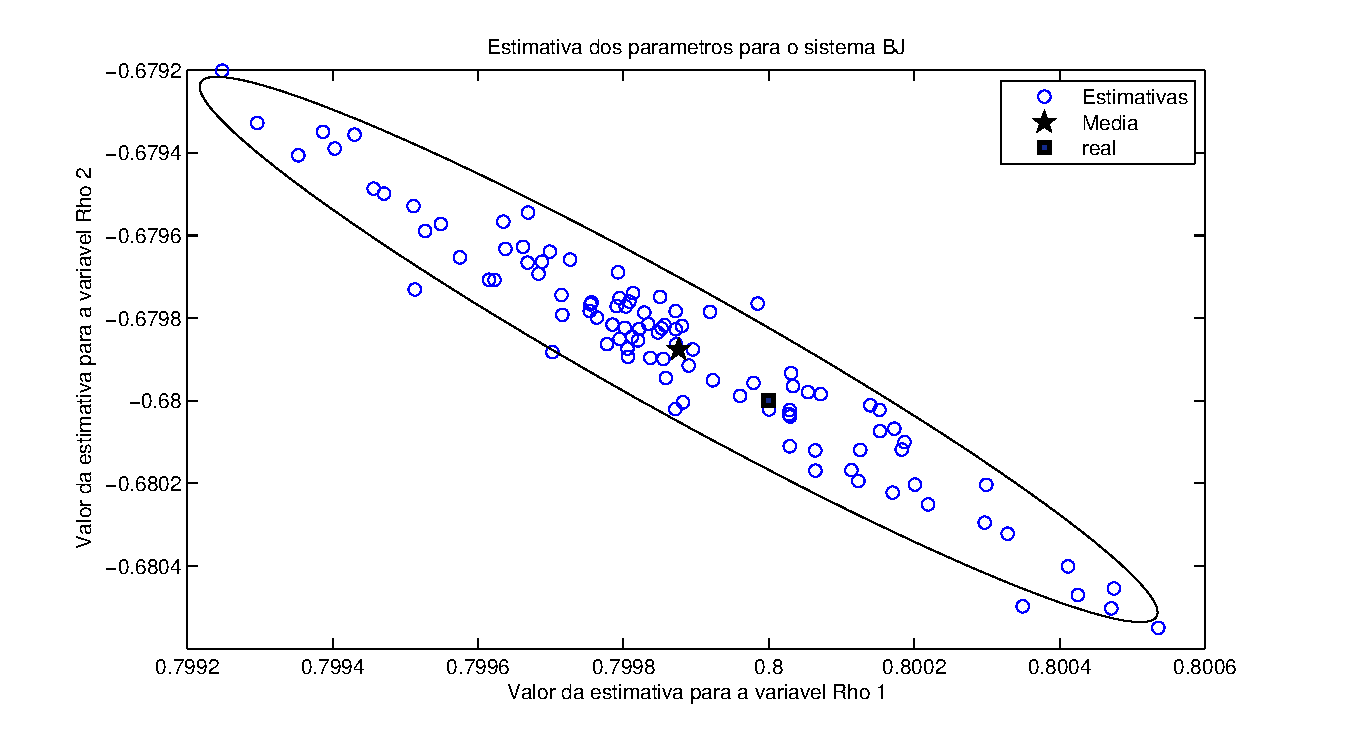
\includegraphics[width=0.95\columnwidth]{figures/vrft_bj_M10_var005.eps}
	\caption{100 estimativas Monte Carlo dos parametros $\rho_1$ e $\rho_2$ para o
	controlador apresentado em \eqref{eq:vrft_methos_ex_bj_c}}
	\label{fig:vrft_bj_M10_var005}
\end{figure}

Os parametros reais esperados para o controlador (equa��o \eqref{eq:vrft_methos_ex_bj_cd}) e a m�dia de todas
as estimativas (valor representado por uma estrela na Figura (\ref{fig:vrft_bj_M10_var005})) n�o s�o os
mesmos. Em uma situa��o onde o erro de polariza��o das estimativas n�o existe, o aumento de N (n�mero de
amostras) implica que esta diferen�a diminui, tendendo a zero. Em um cen�rio onde h� erro de polariza��o, se 
aumentarmos a vari�ncia do ruido do sistema, ser� observado um aumento desta diferen�a.

Na figura (\ref{fig:vrft_bj_M10_var02}) quadruplicou-se a vari�ncia do ruido inserido no sistema ($\sigma
_\upsilon ^2=0.02$). Observa-se ent�o que o erro de polariza��o existe na estimativa. Como descrito em
\cite{campi_leccini_savaresi2002} quando o m�todo do VRFT � utilizado com ruido nas amostras, a estimativa �
inevitavelmente polarizada. Neste mesmo trabalho � sugerido a utiliza��o de {\it{variaveis instrumentais}}
(Se��o (\ref{sec:si_par_estim_iv})) para que este erro de polariza��o seja minimizado.

\begin{figure}[htbp] 
	\center 
	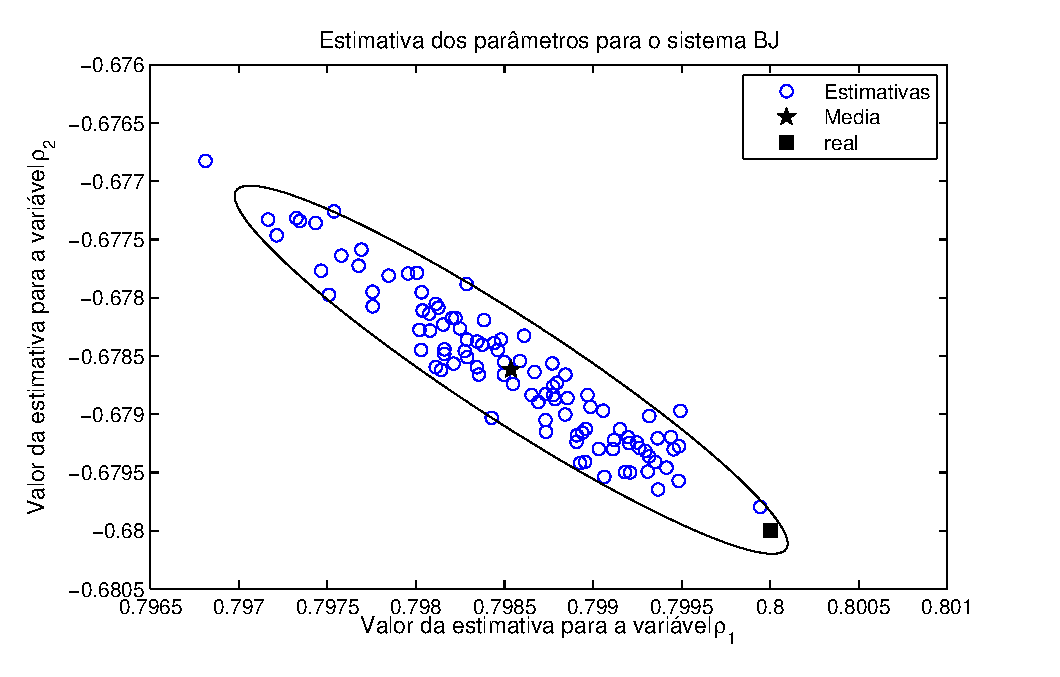
\includegraphics[width=0.95\columnwidth]{figures/vrft_bj_M10_var02.eps}
	\caption{100 estimativas Monte Carlo dos parametros $\rho_1$ e $\rho_2$ para o controlador apresentado em
	\eqref{eq:vrft_methos_ex_bj_c} com varancia do ruido de 0.02}
	\label{fig:vrft_bj_M10_var02}
\end{figure}

Utilizando o procedimento descrito na se��o (\ref{sec:vrft_framework_noise}) para dados corrompidos por ruido
o resultado obtido, para a mesma vari�ncia de $\sigma_\upsilon ^2=0.02$ do ruido, � apresentado na Figura
(\ref{fig:vrft_bj_M10_var02}).

\begin{figure}[htbp]
	\center
	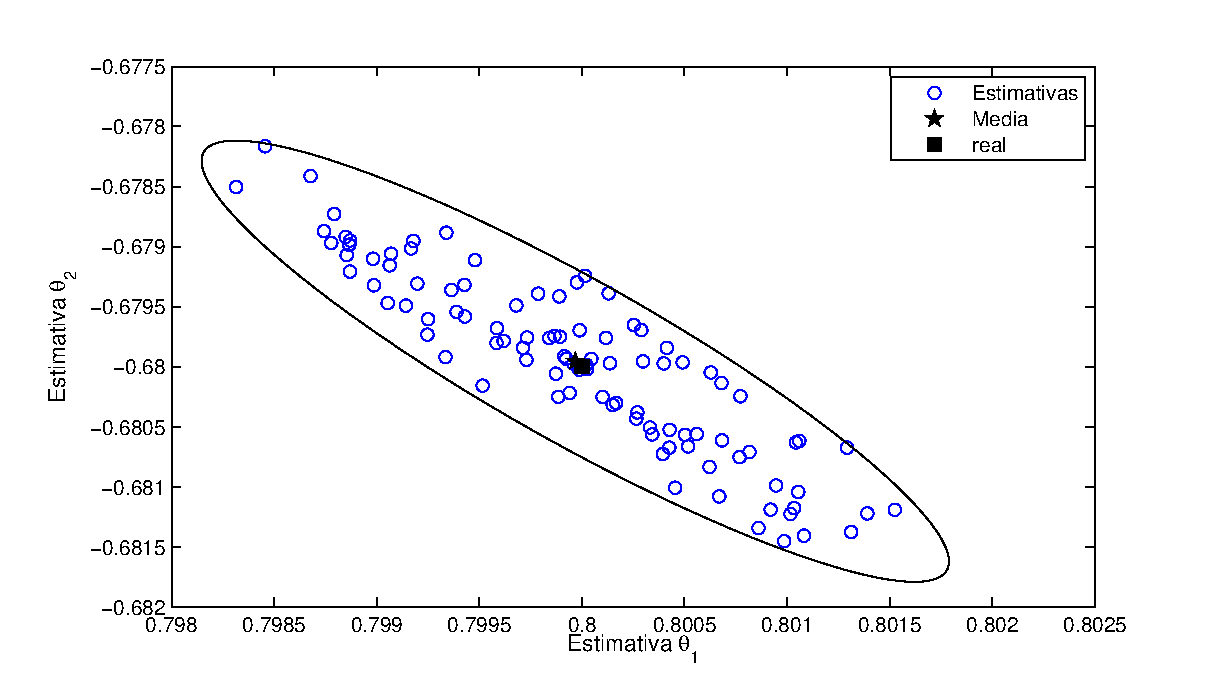
\includegraphics[width=0.95\columnwidth]{figures/vrft_bj_M10_var02_iv.eps}
	\caption{100 estimativas Monte Carlo dos parametros $\rho_1$ e $\rho_2$ para o
	controlador apresentado em \eqref{eq:vrft_methos_ex_bj_c} com varancia do
	ruido de 0.02. Utilizando vari�veis instrumentais para estimar os parametros.}
	\label{fig:vrft_bj_M10_var02_iv}
\end{figure}

Observa-se que o erro de polariza��o foi minimizado e que o resultado obtido possui um custo $J_{VR}^N(\theta)
= 5.1242$ e a vari�ncia dos parametros estimados foi de $0.5064e-06$ para $\rho_1$ e de $0.5495e-06$ para
$\rho_2$.

A fim de comparar o metodo VRFT utilizando e n�o utilizando variaveis instrumentais s�o apresentados abaixo as
Tabelas (\ref{table:vrft_method_bj}) e (\ref{table:vrft_method_bj_iv}) onde o custo $J_{MR}$ (equa��o
\eqref{eq:vrft_method_cost_func}) e o custo $J_{VR}^N$ (equa��o \eqref{eq:vrft_method_filter_criter_assim})
s�o apresentados para diferentes valores de vari�ncia do ruido para o mesmo sismtema BJ.

\begin{table*}[htbp]
\begin{center}
\caption{Valor dos custos $J_{VR}^N$ e $J_{MR}$ al�m da  vari�ncia das
estimativas para diferentes valores de $\sigma _\upsilon ^2$ quando o metodo
VRFT n�o utiliza vari�veis instrumentais para a estimativa dos parametros
$\rho$}
\label{table:vrft_method_bj}
\begin{tabular}{cccc}
\hline
        Vari�ncia $\sigma _\upsilon ^2$ & $J_{VR}^N(\theta)$ &
        $J_{MR}(\theta)$ & Vari�ncia estimativas $\rho$   \\
\hline
	    0.06    & 1.7893e-2 & 8.2367e-3 & 1.0e-05\;[0.4754    0.4434] \\
	    0.05    & 1.2515e-2 & 5.5366e-3 & 1.0e-05\;[0.2671    0.3244] \\
        0.04    & 8.1897e-3 & 3.6071e-3 & 1.0e-05\;[0.1534    0.1583] \\
        0.01    & 4.9665e-4 & 2.4402e-4 & 1.0e-06\;[0.0963    0.1035] \\
        0.005   & 1.2515e-4 & 5.6013e-5 & 1.0e-07\;[0.2999    0.3114] \\
        0.001   & 5.0036e-6 & 3.5734e-6 & 1.0e-08\;[0.1301    0.1223] \\
\hline
\end{tabular}
\end{center}
\end{table*} 
   

\begin{table*}[htbp]
\begin{center}
\caption{Valor dos custos $J_{VR}^N$ e $J_{MR}$ al�m da  vari�ncia das
estimativas para diferentes valores de $\sigma _\upsilon ^2$ quando o metodo
VRFT utiliza vari�veis instrumentais para a estimativa dos parametros $\rho$}
\label{table:vrft_method_bj_iv}
\begin{tabular}{cccc}
\hline
        Vari�ncia $\sigma _\upsilon ^2$ & $J_{VR}^N(\theta)$ &
        $J_{MR}(\theta)$ & Vari�ncia estimativas $\rho$   \\
\hline
	    0.06    & 45.1719  &  9.7345e-05 & 1.0e-05\;[0.5161    0.5332] \\
	    0.05    & 33.2600  &  2.0457e-05 & 1.0e-05\;[0.2481    0.2652] \\
        0.04    & 21.2652  &  1.1665e-04 & 1.0e-05\;[0.2040    0.2084] \\
        0.01    & 1.2956   &  8.9695e-06 & 1.0e-06\;[0.1246    0.1138] \\
        0.005   & 0.3264   &  7.4764e-06 & 1.0e-07\;[0.3063    0.2917] \\
        0.001   & 0.0126   &  5.2443e-07 & 1.0e-08\;[0.1059    0.1017] \\
\hline
\end{tabular}
\end{center}
\end{table*}

Utilizando vari�veis instrumentais observa-se que o custo $J_{MR}(\theta)$ � significativamente mais baixo
quando comparado com o metodo onde n�o s�o utilizadas vari�veis instrumentais. Demonstrando assim que o
comportamento desejado do sistema foi atingido com uma melhor aproxima��o.

%===============================================================================
\subsubsection{Controlador PID - sistema ARX}
\label{sec:vrft_examples_pid_arx}
%===============================================================================

Para um sistema {\it{ARX}} onde $G_0(z)$ e $H_0(z)$ podem ser definidos como:

\begin{equation}
G_{ 0 }(z)=\frac { z }{ (z-0.9)(z-0.8) } ,\quad \quad \quad H_{ 0 }(z)=\frac { z^2 }{ (z-0.9)(z-0.8) } 
\nonumber
\end{equation}

Deseja-se que o sistema em malha fechada comporte-se o mais pr�ximo poss�vel do modelo apresentado em
\eqref{eq:vrft_methos_ex_arx_M}.

\begin{equation}
M(z)=\frac { 0.4 }{ z-0.6 }
\label{eq:vrft_methos_ex_arx_M}
\end{equation}

Tem-se assim que o controlador ideal, aquele que ao ser inserido no sistema em
malha fechada apresentado na Figura (\ref{fig:vrft_db_control_loop}) propicia o
comportamento descrito por \eqref{eq:vrft_methos_ex_arx_M} �:

\begin{equation}
C_d(z)=\frac { 0.4(z - 0.9)(z-0.8) }{ z(z-1) }
\label{eq:vrft_methos_ex_arx_cd}
\end{equation}

Observa-se que este controlador pode ser representado como um controlador
{\it{PID}} como em \eqref{eq:vrft_methos_ex_arx_c}. 

\begin{equation}
C(z,\rho )=\frac { \rho _{ 1 }z^2+\rho _{ 2 }z+\rho _{ 3 } }{ z(z-1) } 
\label{eq:vrft_methos_ex_arx_c}
\end{equation}

Na Figura (\ref{fig:vrft_arx_M10_var005}) � apresentado o resultado da estimativa dos parametros do
controlador quando n�o s�o utilizados variaveis instrumentais. Obteve-se desta forma um custo
$J_{VR}^N(\theta) = 2.5008e-05$ e $J_{MR}(\theta) = 1.7746e-05$ al�m de uma vari�ncia para as estimativas de
$1.0e-07 \; [0.0364\;    0.1261\;    0.0377]$ para $\rho_1$, $\rho_2$ e $\rho_3$ respectivamente.

\begin{figure}[htbp] 
	\center 
	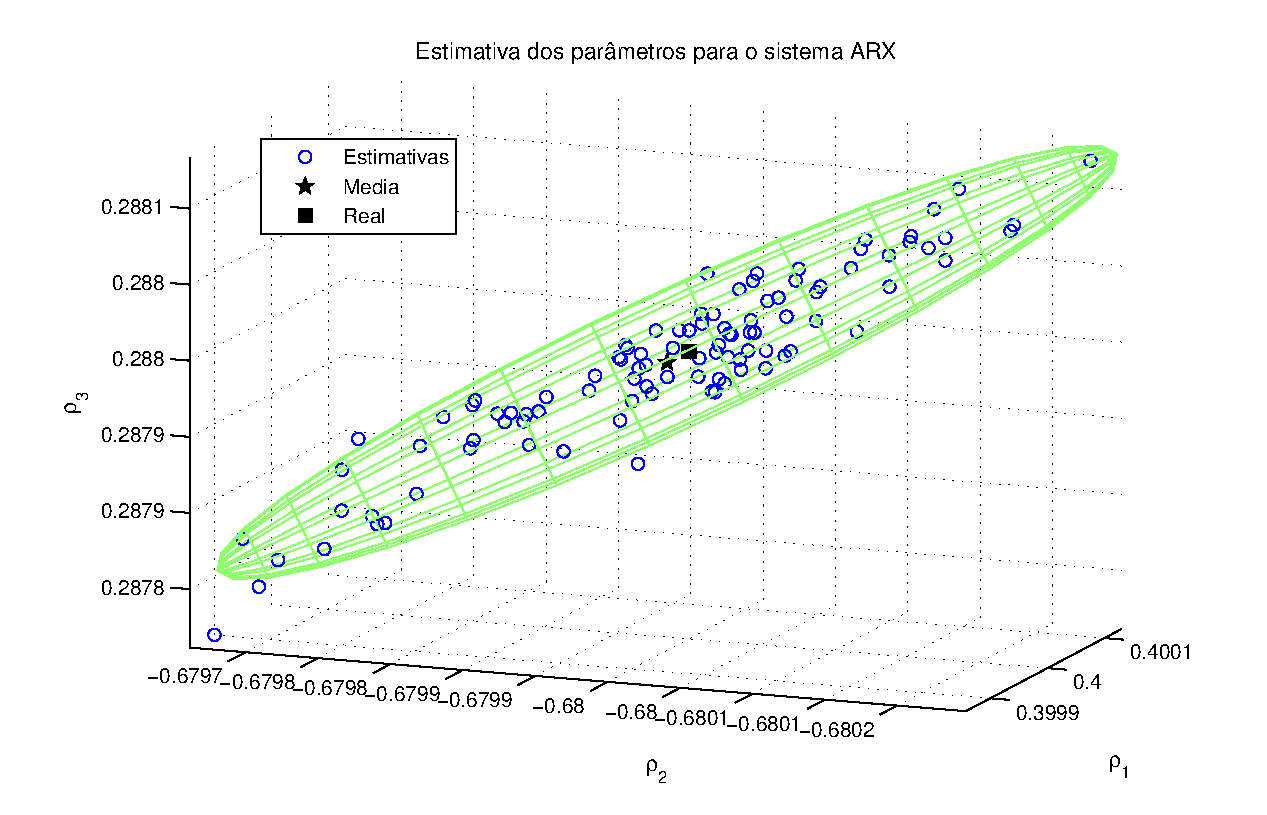
\includegraphics[width=0.95\columnwidth]{figures/vrft_arx_M10_var005_.eps}
	\caption{100 estimativas Monte Carlo dos parametros $\rho_1$, $\rho_2$ e $\rho_3$ para o controlador
	apresentado em \eqref{eq:vrft_methos_ex_arx_c} com varancia do ruido $\sigma_\upsilon ^2=0.005$}
	\label{fig:vrft_arx_M10_var005}
\end{figure}

Como j� foi observado a utiliza��o de variaveis instrumentais melhora significativamente o erro existente nas
estimativas. Desta forma as informa��es apresentadas a seguir ser�o feitas utilizando variaveis instrumentais.
Na figura (\ref{fig:vrft_arx_M10_var05_iv}) � apresentado a estimativa dos parametros do controlador para um
ruido com vari�ncia $\sigma_\upsilon ^2=0.05$. Observa-se que n�o h� erro de polariza��o nas estimativas. 
O custo para esta, e outas, estimativas � apresentado na Tabela (\ref{table:vrft_method_arx_iv}).

\begin{figure}[htbp] 
	\center 
	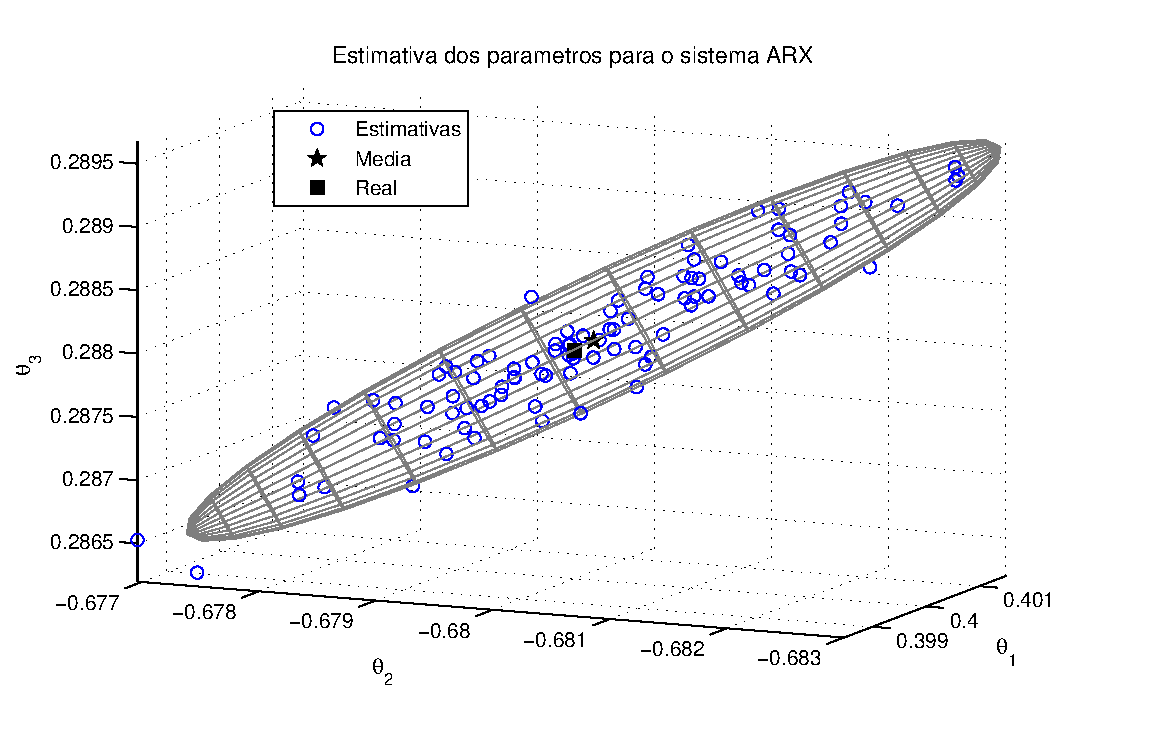
\includegraphics[width=0.95\columnwidth]{figures/vrft_arx_M10_var05_iv.eps}
	\caption{100 estimativas Monte Carlo dos parametros $\rho_1$, $\rho_2$ e $\rho_3$ para o controlador
	apresentado em \eqref{eq:vrft_methos_ex_arx_c} com varancia do ruido $\sigma_\upsilon ^2=0.05$ utilizando
	vari�veis instrumentais}
	\label{fig:vrft_arx_M10_var05_iv}
\end{figure}


\begin{table*}[htbp]
\begin{center}
\caption{Valor dos custos $J_{VR}^N$ e $J_{MR}$ al�m da  vari�ncia das
estimativas para diferentes valores de $\sigma _\upsilon ^2$ quando o metodo
VRFT utiliza vari�veis instrumentais para a estimativa dos parametros $\rho$ do controlador
\eqref{eq:vrft_methos_ex_arx_c}}
\label{table:vrft_method_arx_iv}
\begin{tabular}{cccc}
\hline
        Vari�ncia $\sigma _\upsilon ^2$ & $J_{VR}^N(\theta)$ &
        $J_{MR}(\theta)$ & Vari�ncia estimativas $\rho$   \\
\hline
	    0.1     & 10.0743e-3 & 2.2871e-3  & 1.0e-05\;[0.1253    0.4683    0.1600] \\
	    0.06    & 3.6093e-3  & 1.1279e-3  & 1.0e-05\;[0.0516    0.1793    0.0575] \\
	    0.05    & 2.5419e-3  & 1.2453e-3  & 1.0e-05\;[0.0344    0.1237    0.0416] \\
	    0.04    & 1.6013e-3  & 0.5106e-3  & 1.0e-06\;[0.2195    0.7908    0.2379] \\
        0.01    & 10.0077e-5 & 13.7142e-5 & 1.0e-07\;[0.1552    0.5469    0.1822] \\
        0.005   & 2.5081e-5  & 10.3482e-5 & 1.0e-07\;[0.0406    0.1260    0.0375] \\
		0.001   & 0.1009e-5  & 2.0487e-5  & 1.0e-09\;[0.1277    0.4035    0.1239]
\end{tabular}
\end{center}
\end{table*}

%===============================================================================
\subsubsection{Controlador n�o pertence a classe}
\label{sec:vrft_examples_not_in_class}
%===============================================================================


%===============================================================================
\subsection{VRFT em sistemas n�o lineares}
\label{sec:vrft_nonlinear}
%===============================================================================
ref: \cite{campi_savaresi2006}

\cite{lecchini_campi_savaresi_2dof}


\cite{Guardabassi}














































%===============================================================================
\section{Considera��es Finais}
\label{sec:vrft_conclusions}
%===============================================================================


%===============================================================================


%===============================================================================
\chapter{Identifica��o de sistemas n�o lineares}
\label{chapter:non_linear_sis_ident}
%===============================================================================

%===============================================================================
%===============================================================================
\section{Lineariza��o de sistemas}
\label{sec:non_linear_si_linearization}
%===============================================================================

Talvez o mais comum uso de sistemas lineares variantes no tempo esta relacionado
a lineariza��o de sistema n�o lineares em torno de uma trajet�ria. Suponha que
o sistema n�o linear � descrito por:

\begin{equation}
\left\{\begin{matrix}
x(k+1) = f(x(k),u(k))+r(x(k),u(k))w(k)\\ 
y(k)  = h(x(k))+m(x(k),u(k))\upsilon (k)
\end{matrix}\right.
\label{eq:nl_linearization_sys}
\end{equation}


%===============================================================================
\section{Modelos para sistemas n�o lineares}
\label{sec:non_linear_si_models}
%===============================================================================


%===============================================================================
\section{Algoritmos para identifica��o}
\label{sec:non_linear_si_algorithms}
%===============================================================================

%===============================================================================
\subsection{Modelos Racionais}
\label{sec:nl_algorithms_rationals}
% Aguirre 393
% Tese do corr�a - pg 27
%===============================================================================

%===============================================================================
\section{Considera��es Finais}
\label{sec:vrft_conclusions}
%===============================================================================


%===============================================================================


% \chapter{Estado da arte}
% \chapter{Mais estado da arte}
% \chapter{A minha contribui��o}
% \chapter{Prova de que a minha contribui��o � v�lida}
% \chapter{Conclus�o}

% referencias
% Aqui pode ser usado o ambiente padrao `thebibliography'; por�m, fa�a um
% favor a s� mesmo e use o \bibtex\ e o estilo abnt.bst (veja na p�gina do
% UTUG). 

\bibliographystyle{abnt}

%\bibliography{exemplo,modelo} 	% pode-se ter v�rios arquivos .bib separados
\bibliography{disssertacao_neuhaus} 	% pode-se ter v�rios arquivos .bib separados
				% por v�rgulas. Segundo a NBR6023, as
				% refer�ncias devem ser alinhadas apenas a
				% esquerda. � esquisito, mas � assim.

% Ap�ndices
\appendix

% Pode-se ter diversos ap�ndices
\chapter{T�tulo do Ap�ndice}

Nos ap�ndices aparecem textos ou documentos elaborados pelo autor  a fim de
complementar sua argumenta��o sem preju�zo do trabalho. Eles sempre dever�o
estar depois das refer�ncias e antes dos anexos.


% Anexos
\annex

% Pode-se ter diversos anexos
\chapter{T�tulo do Anexo}

J� os anexos ser�o textos, trabalhos e materiais que n�o foram elaborados
pelo autor, mas que servem de comprova��o, fundamenta��o ou ilustra��o dos
argumentos contidos no texto. Neste ponto, deve-se dar especial aten��o �
quest�o dos direitos autorais.

\end{document}
